% lecture13_ro.tex -- GENERATED by build_L13.py from L13_numbers.json; do not edit by hand.
\documentclass[10pt,aspectratio=169,t]{beamer}
% =============================================================================
% nn_preamble.tex -- shared Beamer preamble of Neural Networks and Deep Learning (NN)
% Used by every lecture: lectures/Lk/lecturek.tex does
%   \documentclass[10pt,aspectratio=169,t]{beamer}
%   % =============================================================================
% nn_preamble.tex -- shared Beamer preamble of Neural Networks and Deep Learning (NN)
% Used by every lecture: lectures/Lk/lecturek.tex does
%   \documentclass[10pt,aspectratio=169,t]{beamer}
%   % =============================================================================
% nn_preamble.tex -- shared Beamer preamble of Neural Networks and Deep Learning (NN)
% Used by every lecture: lectures/Lk/lecturek.tex does
%   \documentclass[10pt,aspectratio=169,t]{beamer}
%   \input{../common/nn_preamble}
%   \nnlecture{k}{Lecture title}
% Logos live in lectures/common/logos/, charts in lectures/Lk/charts/.
% Do NOT add \hfuzz / \vfuzz / \hbadness here: overfull boxes must be fixed, not hidden.
% =============================================================================

\usetheme{default}
\setbeamersize{text margin left=7mm, text margin right=7mm}

% ---------------------------------------------------------------- packages
\usepackage[utf8]{inputenc}
\usepackage[T1]{fontenc}
\usepackage{lmodern}
\usepackage{amsmath, amssymb}
\usepackage{mathtools}
\usepackage{bm}
\usepackage{tikz}
\usetikzlibrary{arrows.meta, positioning, calc, shapes.misc}
\usepackage{booktabs}
\usepackage{array}
\usepackage{graphicx}
\usepackage{colortbl}
\usepackage{xcolor}
\usepackage{multicol}
\hypersetup{colorlinks=true, linkcolor=MainBlue, urlcolor=MainBlue, citecolor=MainBlue}
\graphicspath{{../common/logos/}}   % charts are included with their language folder: charts/en/, charts/ro/

% ---------------------------------------------------------------- colours
\definecolor{MainBlue}{RGB}{26, 58, 110}
\definecolor{IDAred}{RGB}{205, 0, 0}
\definecolor{DarkGray}{RGB}{51, 51, 51}
\definecolor{FooterGray}{RGB}{100, 100, 100}
\definecolor{BlockGray}{RGB}{236, 238, 242}
\definecolor{KeynoteGray}{RGB}{218, 218, 218}
\definecolor{Crimson}{RGB}{190, 40, 50}
\definecolor{Forest}{RGB}{30, 110, 50}
\definecolor{Bitter}{RGB}{214, 150, 20}
% chart palette (same hex values and order as lectures/common/nn_plot.py SERIES)
\definecolor{Ser1}{HTML}{2A78D6}
\definecolor{Ser2}{HTML}{EB6834}
\definecolor{Ser3}{HTML}{1BAF7A}
\definecolor{Ser4}{HTML}{EDA100}
\definecolor{Ser5}{HTML}{E87BA4}
\definecolor{Ser6}{HTML}{008300}
\definecolor{Ser7}{HTML}{6250D6}
\definecolor{Ser8}{HTML}{E34948}

\setbeamertemplate{background}{%
  \begin{tikzpicture}[remember picture, overlay]
    \shade[shading=axis, shading angle=315, top color=white, bottom color=KeynoteGray]
      (current page.south west) rectangle (current page.north east);
  \end{tikzpicture}}
\setbeamercolor{background canvas}{bg=}
\setbeamercolor{structure}{fg=MainBlue}
\setbeamercolor{normal text}{fg=DarkGray}
\setbeamercolor{title}{fg=IDAred}
\setbeamercolor{frametitle}{fg=IDAred, bg=}
\setbeamercolor{block title}{bg=MainBlue, fg=white}
\setbeamercolor{block body}{bg=BlockGray, fg=DarkGray}
\setbeamercolor{block title alerted}{bg=Crimson, fg=white}
\setbeamercolor{block body alerted}{bg=Crimson!7, fg=DarkGray}
\setbeamercolor{block title example}{bg=Forest, fg=white}
\setbeamercolor{block body example}{bg=Forest!7, fg=DarkGray}
\setbeamercolor{item}{fg=MainBlue}
\setbeamerfont{frametitle}{size=\large, series=\bfseries}
\setbeamerfont{block title}{size=\small, series=\bfseries}
\setbeamertemplate{blocks}[rounded][shadow=false]
\setbeamertemplate{itemize item}{\color{MainBlue}$\boxdot$}
\setbeamertemplate{itemize subitem}{\color{MainBlue}\scriptsize$\blacktriangleright$}
% compact two-level lists: level 1 = main point, level 2 = details (no text outside bullets)
\setbeamerfont{itemize/enumerate subbody}{size=\footnotesize}
\setlength{\leftmargini}{1.1em}
\setlength{\leftmarginii}{1.1em}
\setbeamertemplate{itemize/enumerate body begin}{\setlength{\topsep}{0pt}\setlength{\partopsep}{0pt}\setlength{\parskip}{0pt}}
\setbeamertemplate{itemize/enumerate subbody begin}{\setlength{\topsep}{0pt}\setlength{\partopsep}{0pt}\setlength{\itemsep}{0pt}\vspace{-0.4ex}}

\setbeamertemplate{enumerate item}{\color{MainBlue}\insertenumlabel.}
\setlength{\leftmargini}{1.3em}
\setlength{\leftmarginii}{1.2em}
\setbeamertemplate{navigation symbols}{}
\setbeamertemplate{section in toc}{\color{MainBlue}$\blacktriangleright$~\inserttocsection}
\setbeamertemplate{caption}{\raggedright\insertcaption\par}
% frame subtitle = precise citation line under the claim title (Weron style)
\setbeamerfont{framesubtitle}{size=\footnotesize}
\setbeamercolor{framesubtitle}{fg=FooterGray}
% outline that reappears at every section with the current section highlighted
\setbeamertemplate{section in toc shaded}[default][35]
\setbeamertemplate{subsection in toc shaded}[default][35]
\setbeamertemplate{subsection in toc}{\leavevmode\leftskip=2.2em\color{DarkGray}\small\inserttocsubsection\par}
\AtBeginSection[]{{\begin{frame}{\txtoutline}\vspace{2mm}\small
  \tableofcontents[currentsection,hideothersubsections]\end{frame}}}

% ---------------------------------------------------------------- head and foot
\setbeamertemplate{headline}{%
  \vskip10pt%
  \hbox to \paperwidth{\hskip0.5cm%
    {\small\color{FooterGray}\renewcommand{\hyperlink}[2]{##2}\insertsectionhead}%
    \hfill\textcolor{FooterGray}{\small\insertframenumber}\hskip0.5cm}%
  \vskip4pt{\color{FooterGray}\hrule height 0.4pt}}
% footer as in the other courses (MFM, SFM): course name on the left, small sparkline on the right
\setbeamertemplate{footline}{%
  {\color{FooterGray}\hrule height 0.4pt}\vskip4pt%
  \hbox to \paperwidth{\hskip0.5cm%
    \textcolor{FooterGray}{\small\txtcourse}%
    \hfill\raisebox{-0.1em}{\begin{tikzpicture}[x=0.08em, y=0.08em, line width=0.4pt]
      \draw[FooterGray] (0,3) -- (1,4) -- (2,3.5) -- (3,5) -- (4,4) -- (5,6) -- (6,5.5) -- (7,4) -- (8,5) -- (9,7) -- (10,6) -- (11,5) -- (12,6.5) -- (13,8) -- (14,7) -- (15,6) -- (16,7.5) -- (17,9) -- (18,8) -- (19,7) -- (20,8.5) -- (21,10) -- (22,9) -- (23,8) -- (24,9.5);
    \end{tikzpicture}}\hskip0.5cm}%
  \vskip6pt}

% ---------------------------------------------------------------- title page
\defbeamertemplate*{title page}{nn}[1][]{%
  \vspace{0.15cm}
  \begin{center}
    \href{https://www.ase.ro}{
\includegraphics[height=0.9cm]{ase_logo.png}}\hspace{0.3cm}%
    \href{https://ipe.ro/new}{
\includegraphics[height=0.9cm]{acad_logo.png}}\hspace{0.3cm}%
    \href{https://theida.net}{
\includegraphics[height=0.9cm]{ida_logo.png}}\hspace{0.3cm}%
    \href{https://blockchain-research-center.com}{
\includegraphics[height=0.9cm]{brc_logo.png}}\hspace{0.3cm}%
    \href{https://www.ai4efin.ase.ro}{
\includegraphics[height=0.9cm]{ai4efin_logo.png}}\hspace{0.3cm}%
    \href{https://www.digital-finance-msca.com}{
\includegraphics[height=0.9cm]{msca_logo.png}}%
  \end{center}
  \vspace{0.45cm}
  \begin{center}
    \begin{minipage}{0.1\textwidth}\centering
      \href{https://quantlet.com}{
\includegraphics[height=0.9cm]{ql_logo.png}}\end{minipage}%
    \begin{minipage}{0.78\textwidth}\centering
      {\Large\bfseries\usebeamercolor[fg]{title}\inserttitle}\par\vspace{0.25cm}
      {\large\usebeamercolor[fg]{title}\insertsubtitle}\end{minipage}%
    \begin{minipage}{0.1\textwidth}\centering
      \href{https://quantinar.com}{
\includegraphics[height=0.9cm]{qr_logo.png}}\end{minipage}
  \end{center}
  \vfill
  \hspace{0.4cm}{\bfseries\insertauthor}\par\vspace{0.12cm}
  \hspace{0.4cm}\begin{minipage}[t]{0.92\textwidth}\raggedright\footnotesize\insertinstitute\end{minipage}
  \par\vspace{0.4cm}}

% ---------------------------------------------------------------- lecture metadata
\newcommand{\nnshort}{}
\newcommand{\nnnb}{notebooks}
\newcommand{\nnrepo}{https://github.com/danpele/NEURAL_BIZ/tree/main}
% language-dependent labels (English default; \nnromanian switches to Romanian, call it before \nnlecture)
\newcommand{\txtcourse}{Neural Networks and Deep Learning}
\newcommand{\txtlecture}{Lecture}
\newcommand{\txtoutline}{Outline}
\newcommand{\txtintuition}{In one sentence:}
\newcommand{\txtjob}{In practice:}
\newcommand{\txttry}{Experiment yourself:}
\newcommand{\txtwhere}{where}
\newcommand{\txtsim}{SIMULATED DATA (teaching illustration)}
\newcommand{\txtnbsuffix}{}
\newcommand{\txtinstitute}{Bucharest University of Economic Studies (ASE), Department of Statistics and Econometrics\\
    Romanian Academy, Institute for Economic Forecasting (IPE)\\
    IDA Institute Digital Assets \textbullet\ AI4EFin \textbullet\ MSCA Digital Finance}
\newcommand{\nnromanian}{%
  \renewcommand{\txtcourse}{Rețele neuronale și deep learning}%
  \renewcommand{\txtlecture}{Cursul}%
  \renewcommand{\txtoutline}{Cuprins}%
  \renewcommand{\txtintuition}{Pe scurt:}%
  \renewcommand{\txtjob}{În practică:}%
  \renewcommand{\txttry}{Exercițiu practic:}%
  \renewcommand{\txtwhere}{unde}%
  \renewcommand{\txtsim}{DATE SIMULATE (doar pentru ilustrare)}%
  \renewcommand{\txtnbsuffix}{\string_ro}%
  \renewcommand{\txtinstitute}{Academia de Studii Economice din București (ASE), Departamentul de Statistică și Econometrie\\
    Academia Română, Institutul de Prognoză Economică (IPE)\\
    IDA Institute Digital Assets \textbullet\ AI4EFin \textbullet\ MSCA Digital Finance}}
\newcommand{\nnlecture}[2]{%
  \renewcommand{\nnshort}{\txtlecture\ #1}%
  \renewcommand{\nnnb}{notebooks/L#1\string_notebook\txtnbsuffix.ipynb}%
  \title[NN]{\txtcourse}%
  \subtitle{\txtlecture\ #1: #2}%
  \author{Prof.\ dr.\ Daniel Traian PELE}%
  \institute{\txtinstitute}%
  \date{}}

% ---------------------------------------------------------------- teaching blocks (one message per frame)
% \intuition{one plain sentence}  ->  formula with every symbol defined  ->  real-data example  ->  \manager{one line}
\newcommand{\intuition}[1]{\begin{itemize}\item {\color{MainBlue}\textbf{\txtintuition}}~#1\end{itemize}\vspace{0.6mm}}
\newcommand{\manager}[1]{\colorbox{Forest!10}{\parbox{\dimexpr\linewidth-2\fboxsep\relax}{\footnotesize
  \begin{itemize}\setlength{\itemsep}{0pt}\item \textbf{\color{Forest}\txtjob}~#1\end{itemize}}}}
% Experiment yourself: pointer to the matching notebook section
\newcommand{\tryit}[1]{{\scriptsize\href{\nnrepo/\nnnb}{%
  \raisebox{-0.15em}{
\includegraphics[height=0.85em]{ql_logo.png}}\,\textbf{\txttry}~\color{MainBlue}#1}}}
% bottom row: manager line (left) + experiment pointer (right), pinned to the bottom of the frame
\newcommand{\bottomrow}[2]{\par\vfill\noindent\begin{minipage}[b]{0.72\linewidth}#1\end{minipage}\hfill
  \begin{minipage}[b]{0.26\linewidth}\raggedleft #2\end{minipage}\par\vspace{0.5mm}}
\newcommand{\where}[1]{{\footnotesize\textbf{\txtwhere}~#1\par}}

% ---------------------------------------------------------------- helpers
% chart source line under a figure: \chartsource{Source ...; period ...}
\newcommand{\chartsource}[1]{\par\vspace{1pt}{\scriptsize\color{FooterGray}#1\par}}
% link to code: \quantlet{label}{path inside the repo}
\newcommand{\quantlet}[2]{\par\vspace{1pt}\hfill\href{\nnrepo/#2}{%
  \raisebox{-0.15em}{
\includegraphics[height=0.75em]{ql_logo.png}}\textcolor{MainBlue}{\scriptsize\ #1}}}
% inline Quantlet link for the bottom-right corner of a frame: \qlink{label}{path inside the repo}
\newcommand{\qlink}[2]{{\scriptsize\href{\nnrepo/#2}{\raisebox{-0.15em}{
\includegraphics[height=0.85em]{ql_logo.png}}\,\textcolor{MainBlue}{#1}}}}
\newcommand{\simlabel}{\colorbox{Crimson!12}{\scriptsize\bfseries\color{Crimson}\txtsim}}
\newcommand{\E}{\mathbb{E}}
\newcommand{\Var}{\operatorname{Var}}
\newcommand{\Cov}{\operatorname{Cov}}
\newcommand{\Corr}{\operatorname{Corr}}
\newcommand{\asinh}{\operatorname{asinh}}
\newcommand{\iid}{\overset{\text{i.i.d.}}{\sim}}
\newcommand{\EUR}{EUR}
% deep-learning notation (Bishop & Bishop, 2024): vectors bold lower case, matrices bold upper case
\newcommand{\R}{\mathbb{R}}
\newcommand{\vx}{\mathbf{x}}
\newcommand{\vy}{\mathbf{y}}
\newcommand{\vz}{\mathbf{z}}
\newcommand{\vh}{\mathbf{h}}
\newcommand{\vw}{\mathbf{w}}
\newcommand{\vb}{\mathbf{b}}
\newcommand{\mW}{\mathbf{W}}
\newcommand{\mX}{\mathbf{X}}
\newcommand{\btheta}{\boldsymbol{\theta}}
\newcommand{\loss}{\mathcal{L}}
\newcommand{\dataset}{\mathcal{D}}
\DeclareMathOperator*{\argmin}{arg\,min}
\DeclareMathOperator*{\argmax}{arg\,max}
\DeclareMathOperator{\softmax}{softmax}
\DeclareMathOperator{\ReLU}{ReLU}
\DeclareMathOperator{\sigm}{\sigma}

%   \nnlecture{k}{Lecture title}
% Logos live in lectures/common/logos/, charts in lectures/Lk/charts/.
% Do NOT add \hfuzz / \vfuzz / \hbadness here: overfull boxes must be fixed, not hidden.
% =============================================================================

\usetheme{default}
\setbeamersize{text margin left=7mm, text margin right=7mm}

% ---------------------------------------------------------------- packages
\usepackage[utf8]{inputenc}
\usepackage[T1]{fontenc}
\usepackage{lmodern}
\usepackage{amsmath, amssymb}
\usepackage{mathtools}
\usepackage{bm}
\usepackage{tikz}
\usetikzlibrary{arrows.meta, positioning, calc, shapes.misc}
\usepackage{booktabs}
\usepackage{array}
\usepackage{graphicx}
\usepackage{colortbl}
\usepackage{xcolor}
\usepackage{multicol}
\hypersetup{colorlinks=true, linkcolor=MainBlue, urlcolor=MainBlue, citecolor=MainBlue}
\graphicspath{{../common/logos/}}   % charts are included with their language folder: charts/en/, charts/ro/

% ---------------------------------------------------------------- colours
\definecolor{MainBlue}{RGB}{26, 58, 110}
\definecolor{IDAred}{RGB}{205, 0, 0}
\definecolor{DarkGray}{RGB}{51, 51, 51}
\definecolor{FooterGray}{RGB}{100, 100, 100}
\definecolor{BlockGray}{RGB}{236, 238, 242}
\definecolor{KeynoteGray}{RGB}{218, 218, 218}
\definecolor{Crimson}{RGB}{190, 40, 50}
\definecolor{Forest}{RGB}{30, 110, 50}
\definecolor{Bitter}{RGB}{214, 150, 20}
% chart palette (same hex values and order as lectures/common/nn_plot.py SERIES)
\definecolor{Ser1}{HTML}{2A78D6}
\definecolor{Ser2}{HTML}{EB6834}
\definecolor{Ser3}{HTML}{1BAF7A}
\definecolor{Ser4}{HTML}{EDA100}
\definecolor{Ser5}{HTML}{E87BA4}
\definecolor{Ser6}{HTML}{008300}
\definecolor{Ser7}{HTML}{6250D6}
\definecolor{Ser8}{HTML}{E34948}

\setbeamertemplate{background}{%
  \begin{tikzpicture}[remember picture, overlay]
    \shade[shading=axis, shading angle=315, top color=white, bottom color=KeynoteGray]
      (current page.south west) rectangle (current page.north east);
  \end{tikzpicture}}
\setbeamercolor{background canvas}{bg=}
\setbeamercolor{structure}{fg=MainBlue}
\setbeamercolor{normal text}{fg=DarkGray}
\setbeamercolor{title}{fg=IDAred}
\setbeamercolor{frametitle}{fg=IDAred, bg=}
\setbeamercolor{block title}{bg=MainBlue, fg=white}
\setbeamercolor{block body}{bg=BlockGray, fg=DarkGray}
\setbeamercolor{block title alerted}{bg=Crimson, fg=white}
\setbeamercolor{block body alerted}{bg=Crimson!7, fg=DarkGray}
\setbeamercolor{block title example}{bg=Forest, fg=white}
\setbeamercolor{block body example}{bg=Forest!7, fg=DarkGray}
\setbeamercolor{item}{fg=MainBlue}
\setbeamerfont{frametitle}{size=\large, series=\bfseries}
\setbeamerfont{block title}{size=\small, series=\bfseries}
\setbeamertemplate{blocks}[rounded][shadow=false]
\setbeamertemplate{itemize item}{\color{MainBlue}$\boxdot$}
\setbeamertemplate{itemize subitem}{\color{MainBlue}\scriptsize$\blacktriangleright$}
% compact two-level lists: level 1 = main point, level 2 = details (no text outside bullets)
\setbeamerfont{itemize/enumerate subbody}{size=\footnotesize}
\setlength{\leftmargini}{1.1em}
\setlength{\leftmarginii}{1.1em}
\setbeamertemplate{itemize/enumerate body begin}{\setlength{\topsep}{0pt}\setlength{\partopsep}{0pt}\setlength{\parskip}{0pt}}
\setbeamertemplate{itemize/enumerate subbody begin}{\setlength{\topsep}{0pt}\setlength{\partopsep}{0pt}\setlength{\itemsep}{0pt}\vspace{-0.4ex}}

\setbeamertemplate{enumerate item}{\color{MainBlue}\insertenumlabel.}
\setlength{\leftmargini}{1.3em}
\setlength{\leftmarginii}{1.2em}
\setbeamertemplate{navigation symbols}{}
\setbeamertemplate{section in toc}{\color{MainBlue}$\blacktriangleright$~\inserttocsection}
\setbeamertemplate{caption}{\raggedright\insertcaption\par}
% frame subtitle = precise citation line under the claim title (Weron style)
\setbeamerfont{framesubtitle}{size=\footnotesize}
\setbeamercolor{framesubtitle}{fg=FooterGray}
% outline that reappears at every section with the current section highlighted
\setbeamertemplate{section in toc shaded}[default][35]
\setbeamertemplate{subsection in toc shaded}[default][35]
\setbeamertemplate{subsection in toc}{\leavevmode\leftskip=2.2em\color{DarkGray}\small\inserttocsubsection\par}
\AtBeginSection[]{{\begin{frame}{\txtoutline}\vspace{2mm}\small
  \tableofcontents[currentsection,hideothersubsections]\end{frame}}}

% ---------------------------------------------------------------- head and foot
\setbeamertemplate{headline}{%
  \vskip10pt%
  \hbox to \paperwidth{\hskip0.5cm%
    {\small\color{FooterGray}\renewcommand{\hyperlink}[2]{##2}\insertsectionhead}%
    \hfill\textcolor{FooterGray}{\small\insertframenumber}\hskip0.5cm}%
  \vskip4pt{\color{FooterGray}\hrule height 0.4pt}}
% footer as in the other courses (MFM, SFM): course name on the left, small sparkline on the right
\setbeamertemplate{footline}{%
  {\color{FooterGray}\hrule height 0.4pt}\vskip4pt%
  \hbox to \paperwidth{\hskip0.5cm%
    \textcolor{FooterGray}{\small\txtcourse}%
    \hfill\raisebox{-0.1em}{\begin{tikzpicture}[x=0.08em, y=0.08em, line width=0.4pt]
      \draw[FooterGray] (0,3) -- (1,4) -- (2,3.5) -- (3,5) -- (4,4) -- (5,6) -- (6,5.5) -- (7,4) -- (8,5) -- (9,7) -- (10,6) -- (11,5) -- (12,6.5) -- (13,8) -- (14,7) -- (15,6) -- (16,7.5) -- (17,9) -- (18,8) -- (19,7) -- (20,8.5) -- (21,10) -- (22,9) -- (23,8) -- (24,9.5);
    \end{tikzpicture}}\hskip0.5cm}%
  \vskip6pt}

% ---------------------------------------------------------------- title page
\defbeamertemplate*{title page}{nn}[1][]{%
  \vspace{0.15cm}
  \begin{center}
    \href{https://www.ase.ro}{
\includegraphics[height=0.9cm]{ase_logo.png}}\hspace{0.3cm}%
    \href{https://ipe.ro/new}{
\includegraphics[height=0.9cm]{acad_logo.png}}\hspace{0.3cm}%
    \href{https://theida.net}{
\includegraphics[height=0.9cm]{ida_logo.png}}\hspace{0.3cm}%
    \href{https://blockchain-research-center.com}{
\includegraphics[height=0.9cm]{brc_logo.png}}\hspace{0.3cm}%
    \href{https://www.ai4efin.ase.ro}{
\includegraphics[height=0.9cm]{ai4efin_logo.png}}\hspace{0.3cm}%
    \href{https://www.digital-finance-msca.com}{
\includegraphics[height=0.9cm]{msca_logo.png}}%
  \end{center}
  \vspace{0.45cm}
  \begin{center}
    \begin{minipage}{0.1\textwidth}\centering
      \href{https://quantlet.com}{
\includegraphics[height=0.9cm]{ql_logo.png}}\end{minipage}%
    \begin{minipage}{0.78\textwidth}\centering
      {\Large\bfseries\usebeamercolor[fg]{title}\inserttitle}\par\vspace{0.25cm}
      {\large\usebeamercolor[fg]{title}\insertsubtitle}\end{minipage}%
    \begin{minipage}{0.1\textwidth}\centering
      \href{https://quantinar.com}{
\includegraphics[height=0.9cm]{qr_logo.png}}\end{minipage}
  \end{center}
  \vfill
  \hspace{0.4cm}{\bfseries\insertauthor}\par\vspace{0.12cm}
  \hspace{0.4cm}\begin{minipage}[t]{0.92\textwidth}\raggedright\footnotesize\insertinstitute\end{minipage}
  \par\vspace{0.4cm}}

% ---------------------------------------------------------------- lecture metadata
\newcommand{\nnshort}{}
\newcommand{\nnnb}{notebooks}
\newcommand{\nnrepo}{https://github.com/danpele/NEURAL_BIZ/tree/main}
% language-dependent labels (English default; \nnromanian switches to Romanian, call it before \nnlecture)
\newcommand{\txtcourse}{Neural Networks and Deep Learning}
\newcommand{\txtlecture}{Lecture}
\newcommand{\txtoutline}{Outline}
\newcommand{\txtintuition}{In one sentence:}
\newcommand{\txtjob}{In practice:}
\newcommand{\txttry}{Experiment yourself:}
\newcommand{\txtwhere}{where}
\newcommand{\txtsim}{SIMULATED DATA (teaching illustration)}
\newcommand{\txtnbsuffix}{}
\newcommand{\txtinstitute}{Bucharest University of Economic Studies (ASE), Department of Statistics and Econometrics\\
    Romanian Academy, Institute for Economic Forecasting (IPE)\\
    IDA Institute Digital Assets \textbullet\ AI4EFin \textbullet\ MSCA Digital Finance}
\newcommand{\nnromanian}{%
  \renewcommand{\txtcourse}{Rețele neuronale și deep learning}%
  \renewcommand{\txtlecture}{Cursul}%
  \renewcommand{\txtoutline}{Cuprins}%
  \renewcommand{\txtintuition}{Pe scurt:}%
  \renewcommand{\txtjob}{În practică:}%
  \renewcommand{\txttry}{Exercițiu practic:}%
  \renewcommand{\txtwhere}{unde}%
  \renewcommand{\txtsim}{DATE SIMULATE (doar pentru ilustrare)}%
  \renewcommand{\txtnbsuffix}{\string_ro}%
  \renewcommand{\txtinstitute}{Academia de Studii Economice din București (ASE), Departamentul de Statistică și Econometrie\\
    Academia Română, Institutul de Prognoză Economică (IPE)\\
    IDA Institute Digital Assets \textbullet\ AI4EFin \textbullet\ MSCA Digital Finance}}
\newcommand{\nnlecture}[2]{%
  \renewcommand{\nnshort}{\txtlecture\ #1}%
  \renewcommand{\nnnb}{notebooks/L#1\string_notebook\txtnbsuffix.ipynb}%
  \title[NN]{\txtcourse}%
  \subtitle{\txtlecture\ #1: #2}%
  \author{Prof.\ dr.\ Daniel Traian PELE}%
  \institute{\txtinstitute}%
  \date{}}

% ---------------------------------------------------------------- teaching blocks (one message per frame)
% \intuition{one plain sentence}  ->  formula with every symbol defined  ->  real-data example  ->  \manager{one line}
\newcommand{\intuition}[1]{\begin{itemize}\item {\color{MainBlue}\textbf{\txtintuition}}~#1\end{itemize}\vspace{0.6mm}}
\newcommand{\manager}[1]{\colorbox{Forest!10}{\parbox{\dimexpr\linewidth-2\fboxsep\relax}{\footnotesize
  \begin{itemize}\setlength{\itemsep}{0pt}\item \textbf{\color{Forest}\txtjob}~#1\end{itemize}}}}
% Experiment yourself: pointer to the matching notebook section
\newcommand{\tryit}[1]{{\scriptsize\href{\nnrepo/\nnnb}{%
  \raisebox{-0.15em}{
\includegraphics[height=0.85em]{ql_logo.png}}\,\textbf{\txttry}~\color{MainBlue}#1}}}
% bottom row: manager line (left) + experiment pointer (right), pinned to the bottom of the frame
\newcommand{\bottomrow}[2]{\par\vfill\noindent\begin{minipage}[b]{0.72\linewidth}#1\end{minipage}\hfill
  \begin{minipage}[b]{0.26\linewidth}\raggedleft #2\end{minipage}\par\vspace{0.5mm}}
\newcommand{\where}[1]{{\footnotesize\textbf{\txtwhere}~#1\par}}

% ---------------------------------------------------------------- helpers
% chart source line under a figure: \chartsource{Source ...; period ...}
\newcommand{\chartsource}[1]{\par\vspace{1pt}{\scriptsize\color{FooterGray}#1\par}}
% link to code: \quantlet{label}{path inside the repo}
\newcommand{\quantlet}[2]{\par\vspace{1pt}\hfill\href{\nnrepo/#2}{%
  \raisebox{-0.15em}{
\includegraphics[height=0.75em]{ql_logo.png}}\textcolor{MainBlue}{\scriptsize\ #1}}}
% inline Quantlet link for the bottom-right corner of a frame: \qlink{label}{path inside the repo}
\newcommand{\qlink}[2]{{\scriptsize\href{\nnrepo/#2}{\raisebox{-0.15em}{
\includegraphics[height=0.85em]{ql_logo.png}}\,\textcolor{MainBlue}{#1}}}}
\newcommand{\simlabel}{\colorbox{Crimson!12}{\scriptsize\bfseries\color{Crimson}\txtsim}}
\newcommand{\E}{\mathbb{E}}
\newcommand{\Var}{\operatorname{Var}}
\newcommand{\Cov}{\operatorname{Cov}}
\newcommand{\Corr}{\operatorname{Corr}}
\newcommand{\asinh}{\operatorname{asinh}}
\newcommand{\iid}{\overset{\text{i.i.d.}}{\sim}}
\newcommand{\EUR}{EUR}
% deep-learning notation (Bishop & Bishop, 2024): vectors bold lower case, matrices bold upper case
\newcommand{\R}{\mathbb{R}}
\newcommand{\vx}{\mathbf{x}}
\newcommand{\vy}{\mathbf{y}}
\newcommand{\vz}{\mathbf{z}}
\newcommand{\vh}{\mathbf{h}}
\newcommand{\vw}{\mathbf{w}}
\newcommand{\vb}{\mathbf{b}}
\newcommand{\mW}{\mathbf{W}}
\newcommand{\mX}{\mathbf{X}}
\newcommand{\btheta}{\boldsymbol{\theta}}
\newcommand{\loss}{\mathcal{L}}
\newcommand{\dataset}{\mathcal{D}}
\DeclareMathOperator*{\argmin}{arg\,min}
\DeclareMathOperator*{\argmax}{arg\,max}
\DeclareMathOperator{\softmax}{softmax}
\DeclareMathOperator{\ReLU}{ReLU}
\DeclareMathOperator{\sigm}{\sigma}

%   \nnlecture{k}{Lecture title}
% Logos live in lectures/common/logos/, charts in lectures/Lk/charts/.
% Do NOT add \hfuzz / \vfuzz / \hbadness here: overfull boxes must be fixed, not hidden.
% =============================================================================

\usetheme{default}
\setbeamersize{text margin left=7mm, text margin right=7mm}

% ---------------------------------------------------------------- packages
\usepackage[utf8]{inputenc}
\usepackage[T1]{fontenc}
\usepackage{lmodern}
\usepackage{amsmath, amssymb}
\usepackage{mathtools}
\usepackage{bm}
\usepackage{tikz}
\usetikzlibrary{arrows.meta, positioning, calc, shapes.misc}
\usepackage{booktabs}
\usepackage{array}
\usepackage{graphicx}
\usepackage{colortbl}
\usepackage{xcolor}
\usepackage{multicol}
\hypersetup{colorlinks=true, linkcolor=MainBlue, urlcolor=MainBlue, citecolor=MainBlue}
\graphicspath{{../common/logos/}}   % charts are included with their language folder: charts/en/, charts/ro/

% ---------------------------------------------------------------- colours
\definecolor{MainBlue}{RGB}{26, 58, 110}
\definecolor{IDAred}{RGB}{205, 0, 0}
\definecolor{DarkGray}{RGB}{51, 51, 51}
\definecolor{FooterGray}{RGB}{100, 100, 100}
\definecolor{BlockGray}{RGB}{236, 238, 242}
\definecolor{KeynoteGray}{RGB}{218, 218, 218}
\definecolor{Crimson}{RGB}{190, 40, 50}
\definecolor{Forest}{RGB}{30, 110, 50}
\definecolor{Bitter}{RGB}{214, 150, 20}
% chart palette (same hex values and order as lectures/common/nn_plot.py SERIES)
\definecolor{Ser1}{HTML}{2A78D6}
\definecolor{Ser2}{HTML}{EB6834}
\definecolor{Ser3}{HTML}{1BAF7A}
\definecolor{Ser4}{HTML}{EDA100}
\definecolor{Ser5}{HTML}{E87BA4}
\definecolor{Ser6}{HTML}{008300}
\definecolor{Ser7}{HTML}{6250D6}
\definecolor{Ser8}{HTML}{E34948}

\setbeamertemplate{background}{%
  \begin{tikzpicture}[remember picture, overlay]
    \shade[shading=axis, shading angle=315, top color=white, bottom color=KeynoteGray]
      (current page.south west) rectangle (current page.north east);
  \end{tikzpicture}}
\setbeamercolor{background canvas}{bg=}
\setbeamercolor{structure}{fg=MainBlue}
\setbeamercolor{normal text}{fg=DarkGray}
\setbeamercolor{title}{fg=IDAred}
\setbeamercolor{frametitle}{fg=IDAred, bg=}
\setbeamercolor{block title}{bg=MainBlue, fg=white}
\setbeamercolor{block body}{bg=BlockGray, fg=DarkGray}
\setbeamercolor{block title alerted}{bg=Crimson, fg=white}
\setbeamercolor{block body alerted}{bg=Crimson!7, fg=DarkGray}
\setbeamercolor{block title example}{bg=Forest, fg=white}
\setbeamercolor{block body example}{bg=Forest!7, fg=DarkGray}
\setbeamercolor{item}{fg=MainBlue}
\setbeamerfont{frametitle}{size=\large, series=\bfseries}
\setbeamerfont{block title}{size=\small, series=\bfseries}
\setbeamertemplate{blocks}[rounded][shadow=false]
\setbeamertemplate{itemize item}{\color{MainBlue}$\boxdot$}
\setbeamertemplate{itemize subitem}{\color{MainBlue}\scriptsize$\blacktriangleright$}
% compact two-level lists: level 1 = main point, level 2 = details (no text outside bullets)
\setbeamerfont{itemize/enumerate subbody}{size=\footnotesize}
\setlength{\leftmargini}{1.1em}
\setlength{\leftmarginii}{1.1em}
\setbeamertemplate{itemize/enumerate body begin}{\setlength{\topsep}{0pt}\setlength{\partopsep}{0pt}\setlength{\parskip}{0pt}}
\setbeamertemplate{itemize/enumerate subbody begin}{\setlength{\topsep}{0pt}\setlength{\partopsep}{0pt}\setlength{\itemsep}{0pt}\vspace{-0.4ex}}

\setbeamertemplate{enumerate item}{\color{MainBlue}\insertenumlabel.}
\setlength{\leftmargini}{1.3em}
\setlength{\leftmarginii}{1.2em}
\setbeamertemplate{navigation symbols}{}
\setbeamertemplate{section in toc}{\color{MainBlue}$\blacktriangleright$~\inserttocsection}
\setbeamertemplate{caption}{\raggedright\insertcaption\par}
% frame subtitle = precise citation line under the claim title (Weron style)
\setbeamerfont{framesubtitle}{size=\footnotesize}
\setbeamercolor{framesubtitle}{fg=FooterGray}
% outline that reappears at every section with the current section highlighted
\setbeamertemplate{section in toc shaded}[default][35]
\setbeamertemplate{subsection in toc shaded}[default][35]
\setbeamertemplate{subsection in toc}{\leavevmode\leftskip=2.2em\color{DarkGray}\small\inserttocsubsection\par}
\AtBeginSection[]{{\begin{frame}{\txtoutline}\vspace{2mm}\small
  \tableofcontents[currentsection,hideothersubsections]\end{frame}}}

% ---------------------------------------------------------------- head and foot
\setbeamertemplate{headline}{%
  \vskip10pt%
  \hbox to \paperwidth{\hskip0.5cm%
    {\small\color{FooterGray}\renewcommand{\hyperlink}[2]{##2}\insertsectionhead}%
    \hfill\textcolor{FooterGray}{\small\insertframenumber}\hskip0.5cm}%
  \vskip4pt{\color{FooterGray}\hrule height 0.4pt}}
% footer as in the other courses (MFM, SFM): course name on the left, small sparkline on the right
\setbeamertemplate{footline}{%
  {\color{FooterGray}\hrule height 0.4pt}\vskip4pt%
  \hbox to \paperwidth{\hskip0.5cm%
    \textcolor{FooterGray}{\small\txtcourse}%
    \hfill\raisebox{-0.1em}{\begin{tikzpicture}[x=0.08em, y=0.08em, line width=0.4pt]
      \draw[FooterGray] (0,3) -- (1,4) -- (2,3.5) -- (3,5) -- (4,4) -- (5,6) -- (6,5.5) -- (7,4) -- (8,5) -- (9,7) -- (10,6) -- (11,5) -- (12,6.5) -- (13,8) -- (14,7) -- (15,6) -- (16,7.5) -- (17,9) -- (18,8) -- (19,7) -- (20,8.5) -- (21,10) -- (22,9) -- (23,8) -- (24,9.5);
    \end{tikzpicture}}\hskip0.5cm}%
  \vskip6pt}

% ---------------------------------------------------------------- title page
\defbeamertemplate*{title page}{nn}[1][]{%
  \vspace{0.15cm}
  \begin{center}
    \href{https://www.ase.ro}{
\includegraphics[height=0.9cm]{ase_logo.png}}\hspace{0.3cm}%
    \href{https://ipe.ro/new}{
\includegraphics[height=0.9cm]{acad_logo.png}}\hspace{0.3cm}%
    \href{https://theida.net}{
\includegraphics[height=0.9cm]{ida_logo.png}}\hspace{0.3cm}%
    \href{https://blockchain-research-center.com}{
\includegraphics[height=0.9cm]{brc_logo.png}}\hspace{0.3cm}%
    \href{https://www.ai4efin.ase.ro}{
\includegraphics[height=0.9cm]{ai4efin_logo.png}}\hspace{0.3cm}%
    \href{https://www.digital-finance-msca.com}{
\includegraphics[height=0.9cm]{msca_logo.png}}%
  \end{center}
  \vspace{0.45cm}
  \begin{center}
    \begin{minipage}{0.1\textwidth}\centering
      \href{https://quantlet.com}{
\includegraphics[height=0.9cm]{ql_logo.png}}\end{minipage}%
    \begin{minipage}{0.78\textwidth}\centering
      {\Large\bfseries\usebeamercolor[fg]{title}\inserttitle}\par\vspace{0.25cm}
      {\large\usebeamercolor[fg]{title}\insertsubtitle}\end{minipage}%
    \begin{minipage}{0.1\textwidth}\centering
      \href{https://quantinar.com}{
\includegraphics[height=0.9cm]{qr_logo.png}}\end{minipage}
  \end{center}
  \vfill
  \hspace{0.4cm}{\bfseries\insertauthor}\par\vspace{0.12cm}
  \hspace{0.4cm}\begin{minipage}[t]{0.92\textwidth}\raggedright\footnotesize\insertinstitute\end{minipage}
  \par\vspace{0.4cm}}

% ---------------------------------------------------------------- lecture metadata
\newcommand{\nnshort}{}
\newcommand{\nnnb}{notebooks}
\newcommand{\nnrepo}{https://github.com/danpele/NEURAL_BIZ/tree/main}
% language-dependent labels (English default; \nnromanian switches to Romanian, call it before \nnlecture)
\newcommand{\txtcourse}{Neural Networks and Deep Learning}
\newcommand{\txtlecture}{Lecture}
\newcommand{\txtoutline}{Outline}
\newcommand{\txtintuition}{In one sentence:}
\newcommand{\txtjob}{In practice:}
\newcommand{\txttry}{Experiment yourself:}
\newcommand{\txtwhere}{where}
\newcommand{\txtsim}{SIMULATED DATA (teaching illustration)}
\newcommand{\txtnbsuffix}{}
\newcommand{\txtinstitute}{Bucharest University of Economic Studies (ASE), Department of Statistics and Econometrics\\
    Romanian Academy, Institute for Economic Forecasting (IPE)\\
    IDA Institute Digital Assets \textbullet\ AI4EFin \textbullet\ MSCA Digital Finance}
\newcommand{\nnromanian}{%
  \renewcommand{\txtcourse}{Rețele neuronale și deep learning}%
  \renewcommand{\txtlecture}{Cursul}%
  \renewcommand{\txtoutline}{Cuprins}%
  \renewcommand{\txtintuition}{Pe scurt:}%
  \renewcommand{\txtjob}{În practică:}%
  \renewcommand{\txttry}{Exercițiu practic:}%
  \renewcommand{\txtwhere}{unde}%
  \renewcommand{\txtsim}{DATE SIMULATE (doar pentru ilustrare)}%
  \renewcommand{\txtnbsuffix}{\string_ro}%
  \renewcommand{\txtinstitute}{Academia de Studii Economice din București (ASE), Departamentul de Statistică și Econometrie\\
    Academia Română, Institutul de Prognoză Economică (IPE)\\
    IDA Institute Digital Assets \textbullet\ AI4EFin \textbullet\ MSCA Digital Finance}}
\newcommand{\nnlecture}[2]{%
  \renewcommand{\nnshort}{\txtlecture\ #1}%
  \renewcommand{\nnnb}{notebooks/L#1\string_notebook\txtnbsuffix.ipynb}%
  \title[NN]{\txtcourse}%
  \subtitle{\txtlecture\ #1: #2}%
  \author{Prof.\ dr.\ Daniel Traian PELE}%
  \institute{\txtinstitute}%
  \date{}}

% ---------------------------------------------------------------- teaching blocks (one message per frame)
% \intuition{one plain sentence}  ->  formula with every symbol defined  ->  real-data example  ->  \manager{one line}
\newcommand{\intuition}[1]{\begin{itemize}\item {\color{MainBlue}\textbf{\txtintuition}}~#1\end{itemize}\vspace{0.6mm}}
\newcommand{\manager}[1]{\colorbox{Forest!10}{\parbox{\dimexpr\linewidth-2\fboxsep\relax}{\footnotesize
  \begin{itemize}\setlength{\itemsep}{0pt}\item \textbf{\color{Forest}\txtjob}~#1\end{itemize}}}}
% Experiment yourself: pointer to the matching notebook section
\newcommand{\tryit}[1]{{\scriptsize\href{\nnrepo/\nnnb}{%
  \raisebox{-0.15em}{
\includegraphics[height=0.85em]{ql_logo.png}}\,\textbf{\txttry}~\color{MainBlue}#1}}}
% bottom row: manager line (left) + experiment pointer (right), pinned to the bottom of the frame
\newcommand{\bottomrow}[2]{\par\vfill\noindent\begin{minipage}[b]{0.72\linewidth}#1\end{minipage}\hfill
  \begin{minipage}[b]{0.26\linewidth}\raggedleft #2\end{minipage}\par\vspace{0.5mm}}
\newcommand{\where}[1]{{\footnotesize\textbf{\txtwhere}~#1\par}}

% ---------------------------------------------------------------- helpers
% chart source line under a figure: \chartsource{Source ...; period ...}
\newcommand{\chartsource}[1]{\par\vspace{1pt}{\scriptsize\color{FooterGray}#1\par}}
% link to code: \quantlet{label}{path inside the repo}
\newcommand{\quantlet}[2]{\par\vspace{1pt}\hfill\href{\nnrepo/#2}{%
  \raisebox{-0.15em}{
\includegraphics[height=0.75em]{ql_logo.png}}\textcolor{MainBlue}{\scriptsize\ #1}}}
% inline Quantlet link for the bottom-right corner of a frame: \qlink{label}{path inside the repo}
\newcommand{\qlink}[2]{{\scriptsize\href{\nnrepo/#2}{\raisebox{-0.15em}{
\includegraphics[height=0.85em]{ql_logo.png}}\,\textcolor{MainBlue}{#1}}}}
\newcommand{\simlabel}{\colorbox{Crimson!12}{\scriptsize\bfseries\color{Crimson}\txtsim}}
\newcommand{\E}{\mathbb{E}}
\newcommand{\Var}{\operatorname{Var}}
\newcommand{\Cov}{\operatorname{Cov}}
\newcommand{\Corr}{\operatorname{Corr}}
\newcommand{\asinh}{\operatorname{asinh}}
\newcommand{\iid}{\overset{\text{i.i.d.}}{\sim}}
\newcommand{\EUR}{EUR}
% deep-learning notation (Bishop & Bishop, 2024): vectors bold lower case, matrices bold upper case
\newcommand{\R}{\mathbb{R}}
\newcommand{\vx}{\mathbf{x}}
\newcommand{\vy}{\mathbf{y}}
\newcommand{\vz}{\mathbf{z}}
\newcommand{\vh}{\mathbf{h}}
\newcommand{\vw}{\mathbf{w}}
\newcommand{\vb}{\mathbf{b}}
\newcommand{\mW}{\mathbf{W}}
\newcommand{\mX}{\mathbf{X}}
\newcommand{\btheta}{\boldsymbol{\theta}}
\newcommand{\loss}{\mathcal{L}}
\newcommand{\dataset}{\mathcal{D}}
\DeclareMathOperator*{\argmin}{arg\,min}
\DeclareMathOperator*{\argmax}{arg\,max}
\DeclareMathOperator{\softmax}{softmax}
\DeclareMathOperator{\ReLU}{ReLU}
\DeclareMathOperator{\sigm}{\sigma}

\usepackage[romanian]{babel}
\nnromanian
\nnlecture{13}{Deep learning pentru serii de timp din energie și finanțe; modele fundație pentru serii de timp}
\begin{document}
{\setbeamertemplate{headline}{}\setbeamertemplate{footline}{}
\begin{frame}\titlepage\end{frame}}
% END-FRONT-MATTER

\begin{frame}{Obiectivele cursului}
\small
\begin{itemize}\setlength{\itemsep}{4pt}
  \item Să formulați o problemă de prognoză pentru ziua următoare fără scurgeri de informație: setul de informații la închiderea licitației, originea glisantă, modelele de referință.
  \item Să scrieți și să estimați modelul autoregresiv estimat prin Lasso (LEAR), o rețea neuronală profundă (DNN) cu 24 de ieșiri și analiza prin expansiune în baze neuronale (N-BEATS) pe prețurile din România.
  \item Să explicați cum prognozează modelele fundație pentru serii de timp, Chronos și modelul fundație al Google Research (TimesFM), fără antrenare pe datele noastre și să le testați.
  \item Să comparați prognozele cu testul Diebold--Mariano și să calibrați prognozele probabilistice prin predicție conformală.
  \item Să folosiți un model fundație pentru valoarea expusă la risc și să o testați retrospectiv pe S\&P 500 și Bitcoin.
\end{itemize}
\end{frame}

% BEGIN-ABBR

\begin{frame}{Abrevieri (1/2)}
\small
\vspace{-1mm}\begin{columns}[T,onlytextwidth]
\begin{column}{0.49\textwidth}{\scriptsize\renewcommand{\arraystretch}{0.96}\begin{tabular}{@{}>{\bfseries}l@{\ \ }p{0.74\linewidth}@{}}AIC & criteriul informațional Akaike\\
ASE & Academia de Studii Economice din București\\
CET & ora Europei Centrale\\
CQR & regresie cuantilă conformală\\
DE-LU & zona de ofertare Germania--Luxemburg\\
DeepAR & rețea recurentă autoregresivă profundă (Salinas et al., 2020)\\
DM & testul Diebold--Mariano\\
DNN & rețea neuronală profundă (aici: perceptron multistrat cu 24 de ieșiri)\\
ENTSO-E & Rețeaua europeană a operatorilor de transport și de sistem pentru energie electrică\\
ES & pierderea așteptată în coada distribuției (expected shortfall)\\
EUR & euro\\
GARCH & heteroscedasticitate condiționată autoregresivă generalizată\\\end{tabular}}\end{column}
\begin{column}{0.49\textwidth}{\scriptsize\renewcommand{\arraystretch}{0.96}\begin{tabular}{@{}>{\bfseries}l@{\ \ }p{0.74\linewidth}@{}}HS & simulare istorică\\
HU & Ungaria (zonă de ofertare)\\
IPE & Institutul de Prognoză Economică, Academia Română\\
ISE & Institutul Fraunhofer pentru Sisteme de Energie Solară\\
LEAR & model autoregresiv estimat prin Lasso\\
LLM & model lingvistic mare\\
LR & raportul de verosimilitate\\
LSTM & rețea cu memorie pe termen scurt și lung\\
MAD & abaterea absolută mediană\\
MAE & eroarea absolută medie\\
MAPE & eroarea procentuală absolută medie\\
MLP & perceptron multistrat\\\end{tabular}}\end{column}
\end{columns}
\end{frame}

\begin{frame}{Abrevieri (2/2)}
\small
\vspace{-1mm}\begin{columns}[T,onlytextwidth]
\begin{column}{0.49\textwidth}{\scriptsize\renewcommand{\arraystretch}{0.96}\begin{tabular}{@{}>{\bfseries}l@{\ \ }p{0.74\linewidth}@{}}MW & megawatt\\
MWh & megawatt-oră\\
N-BEATS & analiza prin expansiune în baze neuronale pentru serii de timp\\
OPCOM & operatorul pieței de energie electrică și gaze naturale din România\\
PatchTST & arhitectura transformer pe petice de serie de timp\\\end{tabular}}\end{column}
\begin{column}{0.49\textwidth}{\scriptsize\renewcommand{\arraystretch}{0.96}\begin{tabular}{@{}>{\bfseries}l@{\ \ }p{0.74\linewidth}@{}}ReLU & funcția liniară rectificată\\
RMSE & rădăcina erorii pătratice medii\\
RO & România (zonă de ofertare)\\
TimesFM & modelul fundație pentru serii de timp al Google Research\\
VaR & valoarea expusă la risc (Value-at-Risk)\\\end{tabular}}\end{column}
\end{columns}
\end{frame}

% END-ABBR


\section{Problema de prognoză și datele}

\begin{frame}{Două decizii de afaceri bazate pe prognoze pentru ziua următoare}
\small
\begin{itemize}\setlength{\itemsep}{3pt}
  \item \textbf{Energie: ofertarea pe piața pentru ziua următoare}
    \begin{itemize}\setlength{\itemsep}{0pt}
      \item Un furnizor, un producător hidro sau operatorul unei baterii trimite oferte pentru cele 24 de ore de mîine înainte de ora 12:00, ora Europei Centrale (CET), de azi
      \item Prețul fiecărei ore este stabilit de o singură licitație, cuplată la nivel european; în România o organizează operatorul pieței de energie electrică și gaze naturale (OPCOM)
      \item O eroare de 1 EUR/MWh pe 100 MW timp de 24 de ore costă 2.400 de euro pe zi
    \end{itemize}
  \item \textbf{Finanțe: valoarea expusă la risc (VaR) a unui portofoliu}
    \begin{itemize}\setlength{\itemsep}{0pt}
      \item O bancă raportează zilnic pierderea depășită cu probabilitatea de 1\,\%; regulile Basel numără depășirile
      \item Este o prognoză de cuantilă, nu una punctuală
    \end{itemize}
  \item \textbf{Întrebarea acestui curs}
    \begin{itemize}\setlength{\itemsep}{0pt}
      \item Sînt rețelele antrenate pe datele noastre sau modelele fundație preantrenate pe milioane de alte serii mai bune decît reperele simple?
    \end{itemize}
\end{itemize}
\par\vfill\noindent{\scriptsize\color{FooterGray}(Weron, 2014; Lago et al., 2021)}\par\vspace{0.5mm}
\end{frame}

\begin{frame}{Numai date reale: prețurile și consumul de energie din România, S\&P 500 și Bitcoin}
\small
{\footnotesize\renewcommand{\arraystretch}{1.05}\setlength{\tabcolsep}{4pt}
\begin{tabular}{@{}p{0.34\textwidth}p{0.12\textwidth}p{0.3\textwidth}p{0.17\textwidth}@{}}\toprule
Serie & Frecvență & Sursă & Folosită pentru \\ \midrule
Prețurile pentru ziua următoare: România (RO), Germania--Luxemburg (DE-LU), Ungaria (HU) & orară & energy-charts.info, Institutul Fraunhofer pentru Sisteme de Energie Solară (ISE), din datele burselor și ale Rețelei europene a operatorilor de transport și de sistem pentru energie electrică (ENTSO-E) & prognoza prețului \\
Consumul României & orară & energy-charts.info, ENTSO-E & prognoza consumului \\
S\&P 500, Bitcoin (BTC/USD) & zilnică & Yahoo Finance & valoarea expusă la risc \\
\bottomrule\end{tabular}}
\par\vspace{0.5mm}{\scriptsize \begin{itemize}\setlength{\itemsep}{0pt}
  \item Prețuri din 1 ianuarie 2015 pînă la 31 octombrie 2026: 103\,595 de prețuri orare; anul de test este 1 noiembrie 2025 -- 31 octombrie 2026: 364 de zile complete.
  \item Orele lipsă rămîn lipsă; cele două zile pe an cu schimbarea orei sînt păstrate doar dacă există toate cele 24 de ore.
\end{itemize}}
\end{frame}

\begin{frame}{Media zilnică a prețurilor pentru ziua următoare în România}
\small
\intuition{un model antrenat înainte de 2021 nu a văzut niciodată prețuri ca în 2022; unul antrenat pe 2022 supraestimează prețurile de azi.}
\vspace{-1mm}\[ \bar P_d=\frac{1}{24}\sum_{h=0}^{23}P_{d,h} \]\vspace{-2mm}
\begin{center}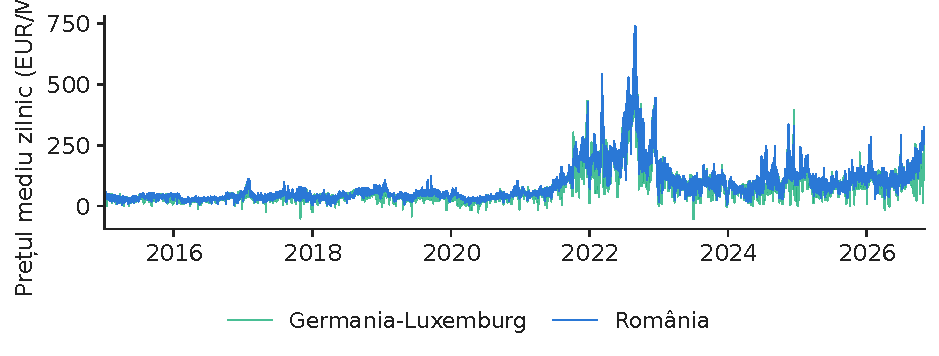
\includegraphics[width=\textwidth,height=0.180\textheight,keepaspectratio]{charts/ro/price_history.pdf}\end{center}\vspace{-3mm}
\chartsource{Sursa: energy-charts.info (Fraunhofer ISE), din datele burselor și ale ENTSO-E. Date: 1 ianuarie 2015 - 31 octombrie 2026, medii zilnice ale prețurilor orare.}
\vspace{0.5mm}
\begin{itemize}\setlength{\itemsep}{0pt}
  \item Media 2019: 50{,}41 EUR/MWh
    \begin{itemize}\setlength{\itemsep}{0pt}
      \item Media 2022: 265{,}31 EUR/MWh
      \item Ziua maximă: 738{,}28, pe 30 august 2022
      \item Corelația mediilor zilnice RO--DE-LU: 0{,}94.
    \end{itemize}
\end{itemize}
\par\vfill\manager{alegeți fereastra de antrenare în mod deliberat: aici, trei ani, ca la Lago et al. (2021).}\par\vspace{0.5mm}
\par\vfill\noindent{\scriptsize\color{FooterGray}}\hfill\qlink{NN\_L13\_price\_history}{Quantlets/L13/NN_L13_price_history}\par\vspace{0.5mm}
\end{frame}

\begin{frame}{Producția solară a transformat vîrful de la prînz într-un minim}
\small
\intuition{forma pe ore este cea mai puternică regularitate pe care o poate învăța un model și s-a schimbat în doar șase ani.}
\vspace{-1mm}\[ \bar P_{\cdot,h}^{(y)}=\frac{1}{|D_y|}\sum_{d\in D_y}P_{d,h} \]\vspace{-2mm}
\begin{center}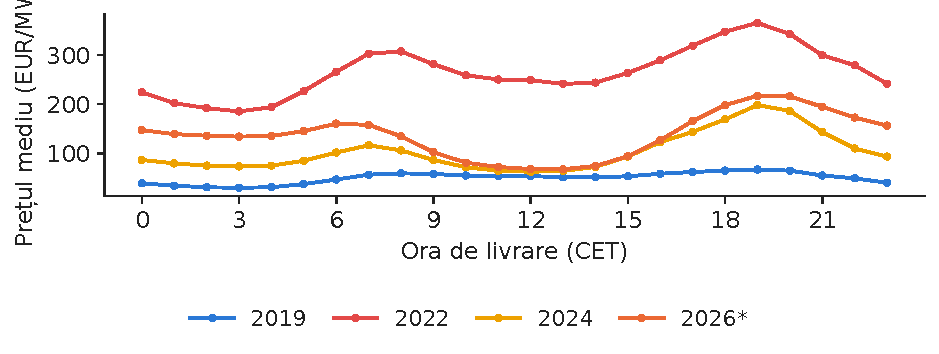
\includegraphics[width=\textwidth,height=0.214\textheight,keepaspectratio]{charts/ro/hourly_profile.pdf}\end{center}\vspace{-3mm}
\chartsource{Sursa: energy-charts.info (Fraunhofer ISE), din datele burselor și ale ENTSO-E. Date: 2019, 2022, 2024 și 2026 (*ianuarie-octombrie), România.}
\vspace{0.5mm}
\begin{itemize}\setlength{\itemsep}{0pt}
  \item 2026 (ianuarie--octombrie): ora cea mai ieftină este 13, cu 67{,}90 EUR/MWh, iar cea mai scumpă este 19, cu 217{,}05 EUR/MWh.
\end{itemize}
\par\vfill\manager{prognoza trebuie să acopere 24 de ore diferite, nu un singur număr pe zi: de aici cele 24 de ieșiri ale modelelor.}\par\vspace{0.5mm}
\par\vfill\noindent{\scriptsize\color{FooterGray}}\hfill\qlink{NN\_L13\_hourly\_profile}{Quantlets/L13/NN_L13_hourly_profile}\par\vspace{0.5mm}
\end{frame}

\begin{frame}{Setul de informații la închiderea licitației: ce poate folosi modelul}
\footnotesize
\intuition{o prognoză pentru ziua $d$ poate folosi doar ce se știe înainte de ora 12:00 CET din ziua $d-1$.}
\begin{columns}[T,onlytextwidth]
\begin{column}{0.53\textwidth}
\[ \hat{\mathbf y}_d=f_{\btheta}(\mathbf x_d),\quad \mathbf x_d\in\mathcal I_{d-1} \]\[ \mathbf x_d=(\mathbf y_{d-1},\mathbf y_{d-2},\mathbf y_{d-3},\mathbf y_{d-7},\mathbf y^{\text{DE}}_{d-1},\boldsymbol\ell_{d-2},\mathbf c_d) \]{\footnotesize\begin{itemize}\setlength{\itemsep}{0pt}
  \item \textbf{\txtwhere}
    \begin{itemize}\setlength{\itemsep}{0pt}
      \item $\mathbf y_d\in\R^{24}$ = prețurile din România în ziua $d$
      \item $\mathbf y^{\text{DE}}$ = prețurile DE-LU
      \item $\boldsymbol\ell$ = consumul României (complet cu două zile în urmă)
      \item $\mathbf c_d$ = variabilele pentru ziua săptămînii
      \item $\mathcal I_{d-1}$ = informația de la închiderea licitației.
    \end{itemize}
\end{itemize}\par}
\end{column}
\begin{column}{0.44\textwidth}
\begin{itemize}\setlength{\itemsep}{2pt}
  \item \textbf{151 de variabile de intrare} și 3\,819 eșantioane zilnice din 2016.
  \item \textbf{Origine glisantă}: reestimare pe ultimele 1\,092 de zile, prognoză pentru ziua următoare, avans cu o zi.
  \item \textbf{Testare o singură dată}: 364 de zile nefolosite nici la estimare, nici la ajustare.
\end{itemize}
\end{column}
\end{columns}
\par\vfill\manager{consumul zilei $d-1$ nu este complet la prînz
    \begin{itemize}\setlength{\itemsep}{0pt}
      \item Folosirea lui ar introduce viitorul în prognoză.
    \end{itemize}}\par\vspace{0.5mm}
\par\vfill\noindent{\scriptsize\color{FooterGray}}\hfill\tryit{notebook \S1}\par\vspace{0.5mm}
\end{frame}

\begin{frame}{Măsurile erorii și modelul de referință}
\footnotesize
\intuition{erorile se raportează în EUR/MWh și relativ la prognoza naivă, niciodată ca procent dintr-un preț care poate fi zero.}
\begin{columns}[T,onlytextwidth]
\begin{column}{0.53\textwidth}
\[ \mathrm{MAE}=\frac{1}{24|\mathcal T|}\sum_{d\in\mathcal T}\sum_{h}|y_{d,h}-\hat y_{d,h}|,\quad \mathrm{rMAE}=\frac{\mathrm{MAE}}{\mathrm{MAE}^{\text{naive}}} \]\[ \hat y^{\text{naive}}_{d,h}=\begin{cases}y_{d-7,h}, & \text{lun., sîm., dum.}\\ y_{d-1,h}, & \text{mar.--vin.}\end{cases} \]{\footnotesize\begin{itemize}\setlength{\itemsep}{0pt}
  \item \textbf{\txtwhere}
    \begin{itemize}\setlength{\itemsep}{0pt}
      \item $\mathcal T$ = zilele de test
      \item $\mathrm{rMAE}<1$ = mai bun decît modelul naiv
      \item Rădăcina erorii pătratice medii (RMSE) ponderează mai mult vîrfurile.
    \end{itemize}
\end{itemize}\par}
\end{column}
\begin{column}{0.44\textwidth}
\begin{itemize}\setlength{\itemsep}{2pt}
  \item \textbf{Anul de test}: media 134{,}59 EUR/MWh, abaterea standard 77{,}19, între \ensuremath{-}97{,}55 și 954{,}59
    \begin{itemize}\setlength{\itemsep}{0pt}
      \item 195 de ore cu preț negativ.
    \end{itemize}
  \item \textbf{Modelul naiv}: eroarea absolută medie (MAE) 27{,}74 EUR/MWh.
\end{itemize}
\end{column}
\end{columns}
\par\vfill\manager{un model cu rMAE peste 1 nu trebuie folosit, oricît de profund ar fi.}\par\vspace{0.5mm}
\par\vfill\noindent{\scriptsize\color{FooterGray}}\hfill\tryit{notebook \S1}\par\vspace{0.5mm}
\end{frame}


\section{Un reper liniar puternic și o rețea profundă}

\begin{frame}{Transformarea care stabilizează varianța: vîrfuri de preț și prețuri negative}
\footnotesize
\intuition{sinusul hiperbolic invers se comportă ca un logaritm pentru prețuri mari și ca identitatea în jurul lui zero, deci acceptă prețuri negative.}
\begin{columns}[T,onlytextwidth]
\begin{column}{0.53\textwidth}
\[ z=\asinh\!\Big(\frac{y-\tilde m}{\hat\sigma}\Big),\quad \hat\sigma=\frac{\mathrm{MAD}}{0.6745},\quad y=\tilde m+\hat\sigma\sinh(\hat z) \]{\footnotesize\begin{itemize}\setlength{\itemsep}{0pt}
  \item \textbf{\txtwhere}
    \begin{itemize}\setlength{\itemsep}{0pt}
      \item $\tilde m$ = mediana ferestrei de antrenare
      \item Abaterea absolută mediană (MAD) scalată la o abatere standard
      \item $\hat z$ = prognoza pe scara transformată.
    \end{itemize}
\end{itemize}\par}
\end{column}
\begin{column}{0.44\textwidth}
\begin{itemize}\setlength{\itemsep}{2pt}
  \item \textbf{Estimată doar pe fereastră}: nicio informație din test nu intră în $\tilde m$ și $\hat\sigma$.
  \item \textbf{Aceeași transformare pentru LEAR și DNN}, astfel încît diferențele vin din model, nu din scară.
\end{itemize}
\end{column}
\end{columns}
\par\vfill\manager{transformați înainte de estimare, inversați după prognoză, evaluați în EUR/MWh.}\par\vspace{0.5mm}
\par\vfill\noindent{\scriptsize\color{FooterGray}(Uniejewski, Weron \& Ziel, 2018)}\hfill\tryit{notebook \S2}\par\vspace{0.5mm}
\end{frame}

\begin{frame}{LEAR: 24 de regresii Lasso, cîte una pentru fiecare oră}
\footnotesize
\intuition{un model liniar cu multe decalaje, în care Lasso păstrează doar decalajele care contează pentru fiecare oră.}
\begin{columns}[T,onlytextwidth]
\begin{column}{0.53\textwidth}
\[ \hat{\boldsymbol\beta}_h=\argmin_{\boldsymbol\beta}\sum_{d\in W}\big(z_{d,h}-\mathbf x_d^{\top}\boldsymbol\beta\big)^2+\lambda_h\lVert\boldsymbol\beta\rVert_1 \]{\footnotesize\begin{itemize}\setlength{\itemsep}{0pt}
  \item \textbf{\txtwhere}
    \begin{itemize}\setlength{\itemsep}{0pt}
      \item $W$ = ultimele 1\,092 de zile
      \item $\lambda_h$ ales prin criteriul informațional Akaike (AIC) pe traiectoria Lasso
      \item Reestimare zilnică: 364 $\times$ 24 de estimări.
    \end{itemize}
\end{itemize}\par}
\end{column}
\begin{column}{0.44\textwidth}
\begin{itemize}\setlength{\itemsep}{2pt}
  \item \textbf{Modelul autoregresiv estimat prin Lasso (LEAR)}: MAE 22{,}79 EUR/MWh, rMAE 0{,}822.
  \item \textbf{De ce este greu de depășit}: se estimează în cîteva secunde, este interpretabil și se adaptează zilnic.
\end{itemize}
\end{column}
\end{columns}
\par\vfill\manager{raportați întotdeauna LEAR lîngă orice rețea: este reperul deschis al domeniului.}\par\vspace{0.5mm}
\par\vfill\noindent{\scriptsize\color{FooterGray}(Lago et al., 2021)}\hfill\tryit{notebook \S2}\par\vspace{0.5mm}
\end{frame}

\begin{frame}{Rețeaua DNN: o singură rețea, 24 de ieșiri, aceleași intrări}
\footnotesize
\intuition{un perceptron multistrat (MLP) prognozează întreaga zi deodată, iar orele împart ce învață.}
\begin{columns}[T,onlytextwidth]
\begin{column}{0.55\textwidth}
\[ \hat{\mathbf z}_d=\mathbf W_3\,\ReLU\big(\mathbf W_2\,\ReLU(\mathbf W_1\mathbf x_d+\mathbf b_1)+\mathbf b_2\big)+\mathbf b_3 \]\[ \loss=\frac{1}{24|W'|}\sum_{d\in W'}\lVert\mathbf z_d-\hat{\mathbf z}_d\rVert_1,\ \ z_{d,h}=\asinh\frac{y_{d,h}-m_d}{s_d} \]{\footnotesize\begin{itemize}\setlength{\itemsep}{0pt}
  \item \textbf{\txtwhere}
    \begin{itemize}\setlength{\itemsep}{0pt}
      \item $m_d$ = mediana prețurilor din ziua $d-1$
      \item $s_d$ = MAD a prețurilor decalate + 1
      \item Funcția liniară rectificată (ReLU)
      \item $W'$ = primele 80\,\% din fereastră.
    \end{itemize}
\end{itemize}\par}
\end{column}
\begin{column}{0.42\textwidth}
\begin{itemize}\setlength{\itemsep}{2pt}
  \item \textbf{Rețeaua neuronală profundă (DNN)}: MAE 23{,}06 EUR/MWh, media a 4 rulări (individual: 23{,}57--24{,}03).
  \item \textbf{Dimensiune}: 256 și 128 de neuroni, 74\,904 parametri, dropout 0{,}1, Adam, oprire timpurie pe ultimele 20\,\%.
  \item \textbf{Scalarea pe fiecare zi} păstrează rețeaua utilizabilă cînd nivelul prețului sare.
\end{itemize}
\end{column}
\end{columns}
\par\vfill\manager{faceți media mai multor rulări
    \begin{itemize}\setlength{\itemsep}{0pt}
      \item O singură rulare este o extragere dintr-un estimator aleator.
    \end{itemize}}\par\vspace{0.5mm}
\par\vfill\noindent{\scriptsize\color{FooterGray}(Lago et al., 2021)}\hfill\tryit{notebook \S3}\par\vspace{0.5mm}
\end{frame}

\begin{frame}{Oprirea timpurie alege epoca pe date pe care rețeaua nu s-a antrenat}
\small
\intuition{pierderea pe antrenare continuă să scadă; pierderea pe validare arată cînd trebuie oprită antrenarea.}
\vspace{-1mm}\[ e^{*}=\argmin_{e}\loss_{\text{val}}(\btheta_e) \]\vspace{-2mm}
\begin{center}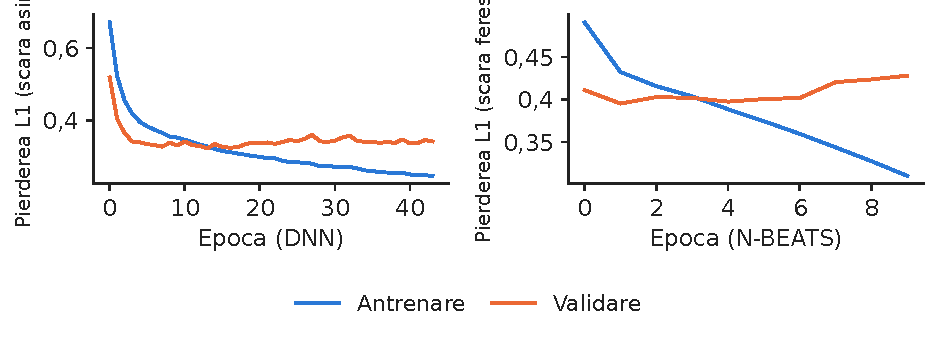
\includegraphics[width=\textwidth,height=0.414\textheight,keepaspectratio]{charts/ro/training_curves.pdf}\end{center}\vspace{-3mm}
\chartsource{Sursa: energy-charts.info (Fraunhofer ISE), din datele burselor și ale ENTSO-E. Date: ferestre de antrenare dinainte de 1 noiembrie 2025, România.}
\vspace{0.5mm}
\begin{itemize}\setlength{\itemsep}{0pt}
  \item DNN: epoca optimă 14 din 44
    \begin{itemize}\setlength{\itemsep}{0pt}
      \item N-BEATS: epoca optimă 2 din 10 (regula răbdării).
    \end{itemize}
\end{itemize}
\par\vfill\noindent{\scriptsize\color{FooterGray}}\hfill\qlink{NN\_L13\_training\_curves}{Quantlets/L13/NN_L13_training_curves}\par\vspace{0.5mm}
\end{frame}


\section{Arhitecturi profunde de prognoză}

\begin{frame}{O rețea recurentă probabilistă pentru prognoză}
\footnotesize
\intuition{starea recurentă rezumă trecutul; rețeaua produce parametrii distribuției de mîine.}
\begin{columns}[T,onlytextwidth]
\begin{column}{0.53\textwidth}
\[ \mathbf h_t=\mathrm{LSTM}(\mathbf h_{t-1},y_{t-1},\mathbf c_t),\quad y_t\mid\mathbf h_t\sim\mathcal N\big(\mu(\mathbf h_t),\sigma^2(\mathbf h_t)\big) \]\[ \loss=-\sum_{t}\log p\big(y_t\mid\mu(\mathbf h_t),\sigma(\mathbf h_t)\big) \]{\footnotesize\begin{itemize}\setlength{\itemsep}{0pt}
  \item \textbf{\txtwhere}
    \begin{itemize}\setlength{\itemsep}{0pt}
      \item Rețea cu memorie pe termen scurt și lung (LSTM, cursul 5)
      \item $\mathbf c_t$ = covariabile
      \item Antrenată simultan pe multe serii înrudite
      \item Prognozele pe mai mulți pași se obțin eșantionînd $y_t$ și reintroducîndu-l în rețea.
    \end{itemize}
\end{itemize}\par}
\end{column}
\begin{column}{0.44\textwidth}
\begin{itemize}\setlength{\itemsep}{2pt}
  \item \textbf{Rețeaua recurentă autoregresivă profundă (DeepAR)}: un singur model global pentru multe serii.
  \item \textbf{Ideea ei continuă} în modelele fundație de mai jos: antrenare globală, prognoză probabilistică.
\end{itemize}
\end{column}
\end{columns}
\par\vfill\manager{este utilă cînd aveți mii de serii înrudite (magazine, contoare, active), nu una singură.}\par\vspace{0.5mm}
\par\vfill\noindent{\scriptsize\color{FooterGray}(Salinas et al., 2020)}\par\vspace{0.5mm}
\end{frame}

\begin{frame}{N-BEATS: blocuri suprapuse care explică intrarea și prognozează restul}
\footnotesize
\intuition{fiecare bloc elimină din intrare ce poate explica (reconstrucția) și adaugă contribuția sa la prognoză.}
\begin{columns}[T,onlytextwidth]
\begin{column}{0.53\textwidth}
\[ \mathbf h_\ell=\mathrm{FC}_\ell(\mathbf r_{\ell-1}),\ \ \hat{\mathbf r}_\ell=\mathbf V^{b}_\ell\mathbf h_\ell,\ \ \hat{\mathbf y}_\ell=\mathbf V^{f}_\ell\mathbf h_\ell \]\[ \mathbf r_\ell=\mathbf r_{\ell-1}-\hat{\mathbf r}_\ell,\qquad \hat{\mathbf y}=\sum_{\ell=1}^{L}\hat{\mathbf y}_\ell \]{\footnotesize\begin{itemize}\setlength{\itemsep}{0pt}
  \item \textbf{\txtwhere}
    \begin{itemize}\setlength{\itemsep}{0pt}
      \item $\mathbf r_0$ = ultimele 168 ore, standardizate pe fereastră
      \item $\mathrm{FC}_\ell$ = 4 straturi de lățime 256
      \item $L$ = 6 blocuri
      \item 1\,739\,904 parametri
      \item Ieșire de 24 de ore.
    \end{itemize}
\end{itemize}\par}
\end{column}
\begin{column}{0.44\textwidth}
\begin{itemize}\setlength{\itemsep}{2pt}
  \item \textbf{Analiza prin expansiune în baze neuronale (N-BEATS)}: doar prețuri, antrenată o singură dată înainte de anul de test, pe toate originile orare.
  \item \textbf{MAE pe test}: 23{,}23 EUR/MWh (3 rulări: între 23{,}69 și 24{,}12).
\end{itemize}
\end{column}
\end{columns}
\par\vfill\manager{o rețea univariată nu vede prețurile din Germania sau consumul: comparați-o cu LEAR, care le folosește.}\par\vspace{0.5mm}
\par\vfill\noindent{\scriptsize\color{FooterGray}(Oreshkin et al., 2020)}\hfill\tryit{notebook \S3}\par\vspace{0.5mm}
\end{frame}

\begin{frame}{Arhitecturi transformer pentru serii de timp: peticele devin tokeni}
\footnotesize
\intuition{seria se taie în petice scurte, fiecare petic este reprezentat ca un cuvînt, iar mecanismul de atenție le compară.}
\begin{columns}[T,onlytextwidth]
\begin{column}{0.53\textwidth}
\[ \mathbf p_j=(y_{(j-1)P+1},\dots,y_{jP}),\quad \mathbf e_j=\mathbf W_{e}\mathbf p_j+\mathbf q_j \]\[ \mathrm{Attn}(\mathbf Q,\mathbf K,\mathbf V)=\softmax\!\Big(\frac{\mathbf Q\mathbf K^{\top}}{\sqrt{d_k}}\Big)\mathbf V \]{\footnotesize\begin{itemize}\setlength{\itemsep}{0pt}
  \item \textbf{\txtwhere}
    \begin{itemize}\setlength{\itemsep}{0pt}
      \item $P$ = lungimea peticului (de exemplu 16 sau 32 de ore)
      \item $\mathbf q_j$ = codificarea poziției
      \item $\mathbf Q,\mathbf K,\mathbf V$ = proiecții ale lui $\mathbf e_j$ (cursul 7).
    \end{itemize}
\end{itemize}\par}
\end{column}
\begin{column}{0.44\textwidth}
\begin{itemize}\setlength{\itemsep}{2pt}
  \item \textbf{Arhitectura transformer pe petice (PatchTST)}: 2.048 de ore devin 128 de tokeni de cîte 16: costul atenției scade de 256 de ori.
  \item \textbf{Modelele fundație} de mai jos folosesc exact acest design, preantrenat pe colecții uriașe de serii.
\end{itemize}
\end{column}
\end{columns}
\par\vfill\manager{peticele fac accesibile contextele lungi (săptămîni de date orare).}\par\vspace{0.5mm}
\par\vfill\noindent{\scriptsize\color{FooterGray}(Nie et al., 2023)}\par\vspace{0.5mm}
\end{frame}


\section{Modele fundație pentru serii de timp}

\begin{frame}{Un model fundație prognozează o serie pe care nu a văzut-o niciodată}
\footnotesize
\intuition{o singură rețea este preantrenată pe multe serii; la utilizare doar citește contextul nostru, fără niciun pas de gradient.}
\begin{columns}[T,onlytextwidth]
\begin{column}{0.53\textwidth}
\[ \hat q^{\tau}_{T+k}=g_{\btheta^{*}}\big(y_{T-C+1:T}\big)_{k,\tau} \]\[ \btheta^{*}=\argmin_{\btheta}\sum_{s\in\mathcal S}\sum_{t,\tau}\rho_\tau\big(y^{(s)}_t-\hat q^{\tau,(s)}_t\big) \]{\footnotesize\begin{itemize}\setlength{\itemsep}{0pt}
  \item \textbf{\txtwhere}
    \begin{itemize}\setlength{\itemsep}{0pt}
      \item $\mathcal S$ = corpusul de preantrenare (serii publice și sintetice)
      \item $C$ = lungimea contextului (aici 2\,048 de ore)
      \item $\rho_\tau$ = pierderea cuantilă (pinball)
      \item $k=1,\dots,24$ = orizontul
      \item $\btheta^{*}$ rămîne fix.
    \end{itemize}
\end{itemize}\par}
\end{column}
\begin{column}{0.44\textwidth}
\begin{itemize}\setlength{\itemsep}{2pt}
  \item \textbf{Trei modele testate, fără reantrenare (zero-shot)}
    \begin{itemize}\setlength{\itemsep}{0pt}
      \item Chronos-2 (Amazon, 2025): covariabile și mai multe serii împreună
      \item Chronos-Bolt base (Amazon): prognoze directe de cuantile
      \item Modelul fundație pentru serii de timp al Google Research (TimesFM) 2.5: numai decodor
    \end{itemize}
\end{itemize}
\end{column}
\end{columns}
\par\vfill\manager{zero-shot înseamnă fără cost de antrenare și fără flux de date, dar și fără adaptare la piața noastră.}\par\vspace{0.5mm}
\par\vfill\noindent{\scriptsize\color{FooterGray}(Ansari et al., 2024, 2025; Das et al., 2024)}\hfill\tryit{notebook \S4}\par\vspace{0.5mm}
\end{frame}

\begin{frame}{Chronos: tokenizarea seriilor de timp}
\footnotesize
\intuition{seria se scalează, valorile se împart în intervale, iar un model de limbaj prezice intervalul următor.}
\begin{columns}[T,onlytextwidth]
\begin{column}{0.53\textwidth}
\[ \tilde y_t=\frac{y_t}{s},\ \ s=\frac{1}{C}\sum_{t}|y_t|,\qquad v_t=\mathrm{bin}(\tilde y_t)\in\{1,\dots,B\} \]\[ \loss=-\sum_{t}\log p_{\btheta}(v_{t+1}\mid v_{1:t}) \]{\footnotesize\begin{itemize}\setlength{\itemsep}{0pt}
  \item \textbf{\txtwhere}
    \begin{itemize}\setlength{\itemsep}{0pt}
      \item $s$ = scara absolută medie a contextului
      \item $B$ = 4.096 de intervale
      \item Modelul este de tip T5
      \item Chronos-Bolt și Chronos-2 folosesc petice și ieșiri de cuantile.
    \end{itemize}
\end{itemize}\par}
\end{column}
\begin{column}{0.44\textwidth}
\begin{itemize}\setlength{\itemsep}{2pt}
  \item \textbf{Scalarea face seriile comparabile}: un preț și un volum de vînzări devin intrări de același tip.
  \item \textbf{Pierderea cuantilă} dă direct prognoze probabilistice.
\end{itemize}
\end{column}
\end{columns}
\par\vfill\manager{modelul cunoaște forme (sezonalitate, revenire la medie), nu piața românească.}\par\vspace{0.5mm}
\par\vfill\noindent{\scriptsize\color{FooterGray}(Ansari et al., 2024)}\par\vspace{0.5mm}
\end{frame}

\begin{frame}{Precizia în anul de test: toate cele nouă prognoze, pe aceleași zile}
\small
\begin{columns}[T,onlytextwidth]
\begin{column}{0.52\textwidth}
{\footnotesize\renewcommand{\arraystretch}{1.05}\setlength{\tabcolsep}{4pt}
\begin{tabular}{@{}lrrr@{}}\toprule
Model & MAE & RMSE & rMAE \\ \midrule
\textbf{Chronos-2 cu covariabile} & \cellcolor{Forest!55}20{,}41 & 33{,}88 & \cellcolor{Forest!55}0{,}736 \\
Chronos-2 & \cellcolor{Forest!50}20{,}72 & 34{,}23 & \cellcolor{Forest!50}0{,}747 \\
ansamblul & \cellcolor{Forest!50}20{,}77 & 34{,}27 & \cellcolor{Forest!49}0{,}749 \\
Chronos-Bolt & \cellcolor{Forest!36}21{,}67 & 34{,}51 & \cellcolor{Forest!36}0{,}781 \\
TimesFM & \cellcolor{Forest!26}22{,}37 & 36{,}08 & \cellcolor{Forest!26}0{,}806 \\
LEAR & \cellcolor{Forest!19}22{,}79 & 36{,}27 & \cellcolor{Forest!19}0{,}822 \\
DNN & \cellcolor{Forest!15}23{,}06 & 38{,}42 & \cellcolor{Forest!15}0{,}831 \\
N-BEATS & \cellcolor{Forest!13}23{,}23 & 36{,}64 & \cellcolor{Forest!13}0{,}837 \\
modelul naiv & \cellcolor{Crimson!55}27{,}74 & 44{,}57 & \cellcolor{Crimson!55}1{,}000 \\
\bottomrule\end{tabular}}
\end{column}
\begin{column}{0.45\textwidth}
\begin{itemize}\setlength{\itemsep}{3pt}
  \item \textbf{Cea mai mică MAE}: Chronos-2 cu covariabile, 20{,}41 EUR/MWh.
  \item \textbf{Cel mai bun model fundație}: Chronos-2 cu covariabile, 20{,}41, mai bun decît LEAR (22{,}79), fără nicio antrenare pe datele noastre.
  \item \textbf{Toate modelele} sînt mai bune decît cel naiv: rMAE sub 1.
  \item Verde = eroare mai mică
    \begin{itemize}\setlength{\itemsep}{0pt}
      \item Semnificația, pe slide-urile următoare.
    \end{itemize}
\end{itemize}
\end{column}
\end{columns}
\par\vfill\noindent{\scriptsize\color{FooterGray}(calcul propriu, EUR/MWh)}\hfill\tryit{notebook \S4}\par\vspace{0.5mm}
\end{frame}

\begin{frame}{Rețele antrenate față de modele fundație fără reantrenare}
\small
\intuition{aceleași 8\,736 de ore, același set de informații, nouă strategii de prognoză.}
\begin{center}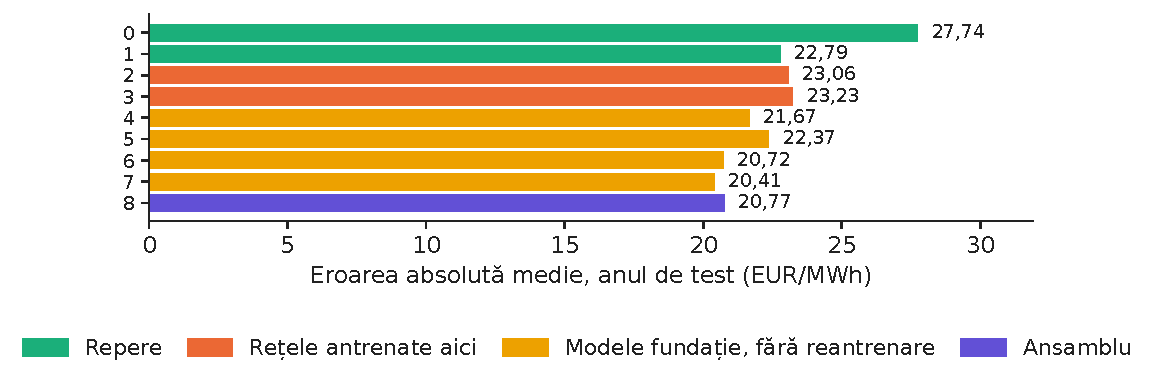
\includegraphics[width=\textwidth,height=0.469\textheight,keepaspectratio]{charts/ro/mae_models.pdf}\end{center}\vspace{-3mm}
\chartsource{Sursa: energy-charts.info (Fraunhofer ISE), din datele burselor și ale ENTSO-E. Date: 1 noiembrie 2025 - 31 octombrie 2026, 360 de zile x 24 de ore, România.}
\vspace{0.5mm}
\begin{itemize}\setlength{\itemsep}{0pt}
  \item Ansamblul = media simplă a LEAR, DNN și Chronos-2: MAE 20{,}77 EUR/MWh.
\end{itemize}
\par\vfill\manager{începeți cu reperul și cu un model fundație: amîndouă costă minute, nu săptămîni.}\par\vspace{0.5mm}
\par\vfill\noindent{\scriptsize\color{FooterGray}}\hfill\qlink{NN\_L13\_mae\_models}{Quantlets/L13/NN_L13_mae_models}\par\vspace{0.5mm}
\end{frame}

\begin{frame}{Erorile sînt cele mai mari seara și în orele cu producție solară}
\small
\intuition{media ascunde orele în care toate modelele greșesc împreună.}
\vspace{-1mm}\[ \mathrm{MAE}_h=\frac{1}{|\mathcal T|}\sum_{d\in\mathcal T}|y_{d,h}-\hat y_{d,h}| \]\vspace{-2mm}
\begin{center}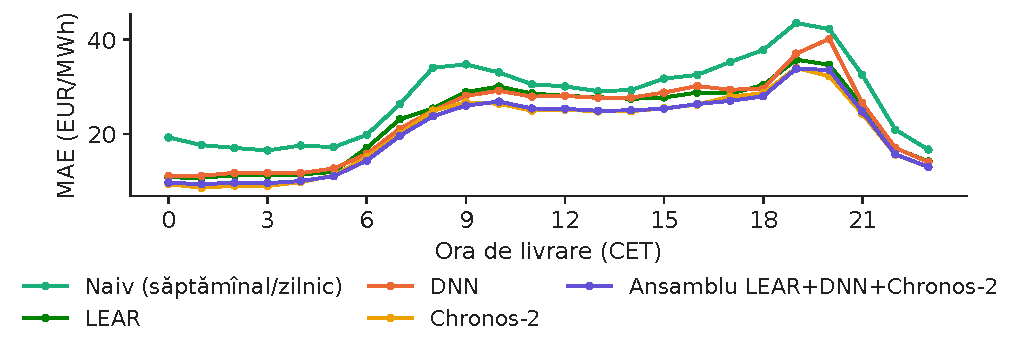
\includegraphics[width=\textwidth,height=0.436\textheight,keepaspectratio]{charts/ro/mae_by_hour.pdf}\end{center}\vspace{-3mm}
\chartsource{Sursa: energy-charts.info (Fraunhofer ISE), din datele burselor și ale ENTSO-E. Date: 1 noiembrie 2025 - 31 octombrie 2026, 360 de zile x 24 de ore, România.}
\vspace{0.5mm}
\begin{itemize}\setlength{\itemsep}{0pt}
  \item LEAR: ora cea mai grea 19 (35{,}78), cea mai ușoară 1 (10{,}75)
    \begin{itemize}\setlength{\itemsep}{0pt}
      \item Chronos-2: ora cea mai grea 19 (34{,}05).
    \end{itemize}
\end{itemize}
\par\vfill\noindent{\scriptsize\color{FooterGray}}\hfill\qlink{NN\_L13\_mae\_by\_hour}{Quantlets/L13/NN_L13_mae_by_hour}\par\vspace{0.5mm}
\end{frame}

\begin{frame}{Prognozele pentru o săptămînă din anul de test}
\small
\intuition{toate cele trei modele urmăresc forma zilnică; niciunul nu anticipează complet cele mai mari vîrfuri de seară.}
\begin{center}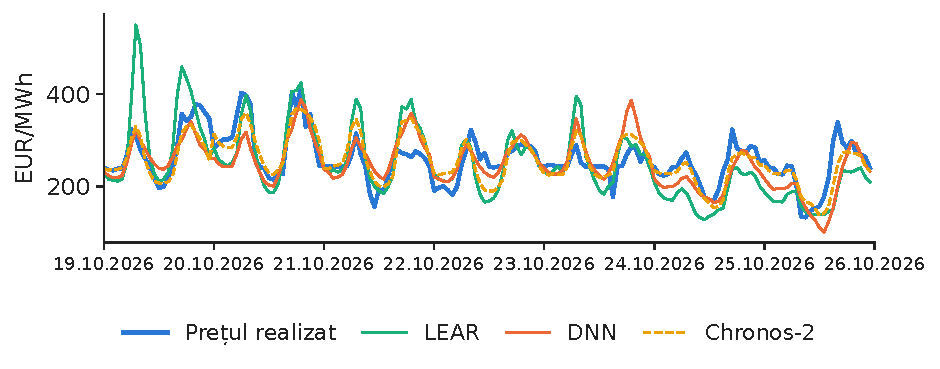
\includegraphics[width=\textwidth,height=0.469\textheight,keepaspectratio]{charts/ro/forecast_week.pdf}\end{center}\vspace{-3mm}
\chartsource{Sursa: energy-charts.info (Fraunhofer ISE), din datele burselor și ale ENTSO-E. Date: 19 octombrie 2026 - 25 octombrie 2026, orar, România.}
\vspace{0.5mm}
\begin{itemize}\setlength{\itemsep}{0pt}
  \item Săptămîna 19 octombrie 2026 -- 25 octombrie 2026: MAE LEAR 43{,}34, DNN 32{,}33, Chronos-2 25{,}41 EUR/MWh.
\end{itemize}
\par\vfill\noindent{\scriptsize\color{FooterGray}}\hfill\qlink{NN\_L13\_forecast\_week}{Quantlets/L13/NN_L13_forecast_week}\par\vspace{0.5mm}
\end{frame}

\begin{frame}{Un context mai lung ajută modelul fundație, pînă la un punct}
\small
\intuition{modelul vede doar contextul: o săptămînă arată forma zilnică, trei luni arată și nivelul.}
\begin{center}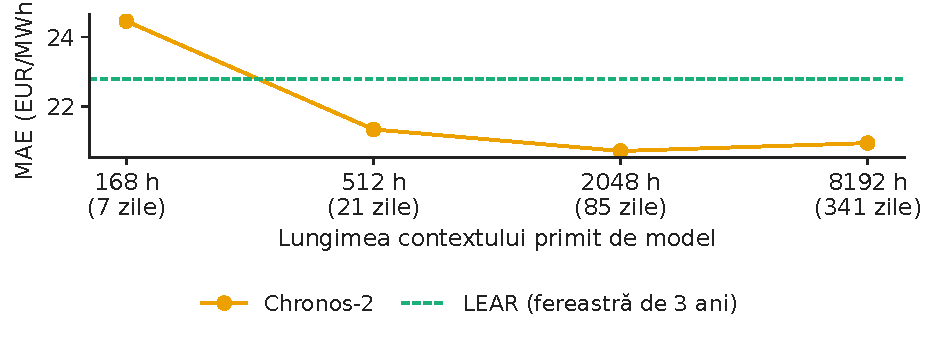
\includegraphics[width=\textwidth,height=0.426\textheight,keepaspectratio]{charts/ro/context_length.pdf}\end{center}\vspace{-3mm}
\chartsource{Sursa: energy-charts.info (Fraunhofer ISE), din datele burselor și ale ENTSO-E. Date: 1 noiembrie 2025 - 31 octombrie 2026, 360 de zile x 24 de ore, România.}
\vspace{0.5mm}
\begin{itemize}\setlength{\itemsep}{0pt}
  \item MAE Chronos-2: 168 h 24{,}45, 512 h 21{,}34, 2.048 h 20{,}72, 8.192 h 20{,}95 EUR/MWh.
\end{itemize}
\par\vfill\manager{lungimea contextului este principalul parametru de ajustare al unui model zero-shot: alegeți-o pe date din trecut.}\par\vspace{0.5mm}
\par\vfill\noindent{\scriptsize\color{FooterGray}}\hfill\qlink{NN\_L13\_context\_length}{Quantlets/L13/NN_L13_context_length}\par\vspace{0.5mm}
\end{frame}

\begin{frame}{Covariabile într-un model fundație: prețurile din Germania și consumul României}
\footnotesize
\intuition{Chronos-2 citește mai multe serii aliniate și lasă mecanismul de atenție să transfere informație între ele.}
\begin{columns}[T,onlytextwidth]
\begin{column}{0.53\textwidth}
\[ \hat{\mathbf q}_{T+1:T+24}=g_{\btheta^{*}}\big(y_{1:T},\ x^{\text{DE}}_{1:T},\ x^{\text{HU}}_{1:T},\ \ell_{1:T}\big) \]{\footnotesize\begin{itemize}\setlength{\itemsep}{0pt}
  \item \textbf{\txtwhere}
    \begin{itemize}\setlength{\itemsep}{0pt}
      \item Covariabile cunoscute doar în trecut: prețurile DE-LU și HU și consumul României pînă la originea prognozei (valorile lor viitoare nu se cunosc la închiderea licitației).
    \end{itemize}
\end{itemize}\par}
\end{column}
\begin{column}{0.44\textwidth}
\begin{itemize}\setlength{\itemsep}{2pt}
  \item \textbf{Fără covariabile}: MAE 20{,}72
    \begin{itemize}\setlength{\itemsep}{0pt}
      \item \textbf{cu covariabile}: 20{,}41 EUR/MWh.
    \end{itemize}
  \item \textbf{Covariabilele au ajutat} aici
    \begin{itemize}\setlength{\itemsep}{0pt}
      \item Testați, nu presupuneți.
    \end{itemize}
\end{itemize}
\end{column}
\end{columns}
\par\vfill\manager{o covariabilă cunoscută dinainte (prognoza meteo sau a consumului) valorează mai mult decît una cunoscută doar în trecut.}\par\vspace{0.5mm}
\par\vfill\noindent{\scriptsize\color{FooterGray}(Ansari et al., 2025)}\hfill\tryit{notebook \S5}\par\vspace{0.5mm}
\end{frame}

\begin{frame}{Testul Diebold--Mariano pe pierderile zilnice}
\footnotesize
\intuition{o eroare medie mai mică poate fi noroc; testăm dacă diferența zilnică a pierderilor are media zero.}
\begin{columns}[T,onlytextwidth]
\begin{column}{0.53\textwidth}
\[ \Delta_d=\lVert\mathbf e^{A}_d\rVert_1-\lVert\mathbf e^{B}_d\rVert_1,\qquad \mathrm{DM}=\frac{\bar\Delta}{\hat\sigma_\Delta/\sqrt{|\mathcal T|}}\ \overset{a}{\sim}\ \mathcal N(0,1) \]{\footnotesize\begin{itemize}\setlength{\itemsep}{0pt}
  \item \textbf{\txtwhere}
    \begin{itemize}\setlength{\itemsep}{0pt}
      \item $\mathbf e^{A}_d\in\R^{24}$ = erorile modelului A în ziua $d$
      \item O statistică pentru fiecare pereche (varianta multivariată)
      \item $H_1$ unilaterală: B este mai precis decît A
      \item $|\mathcal T|$ = 360 de zile.
    \end{itemize}
\end{itemize}\par}
\end{column}
\begin{column}{0.44\textwidth}
\begin{itemize}\setlength{\itemsep}{2pt}
  \item \textbf{Diebold--Mariano (DM)}: LEAR față de DNN, $p$ = 0{,}761
    \begin{itemize}\setlength{\itemsep}{0pt}
      \item LEAR față de Chronos-2, $p$ = $<$0{,}001.
    \end{itemize}
  \item \textbf{Pe zile, nu pe ore}: orele aceleiași zile folosesc aceeași informație, deci nu sînt independente.
\end{itemize}
\end{column}
\end{columns}
\par\vfill\manager{afirmați că un model este mai bun doar pe baza unui test pe perioada de test.}\par\vspace{0.5mm}
\par\vfill\noindent{\scriptsize\color{FooterGray}(Diebold \& Mariano, 1995; Ziel \& Weron, 2018)}\hfill\tryit{notebook \S6}\par\vspace{0.5mm}
\end{frame}

\begin{frame}{Testele Diebold--Mariano pe perechi de modele}
\small
\intuition{celulele verzi: modelul din coloană este semnificativ mai precis decît cel din rînd.}
\begin{center}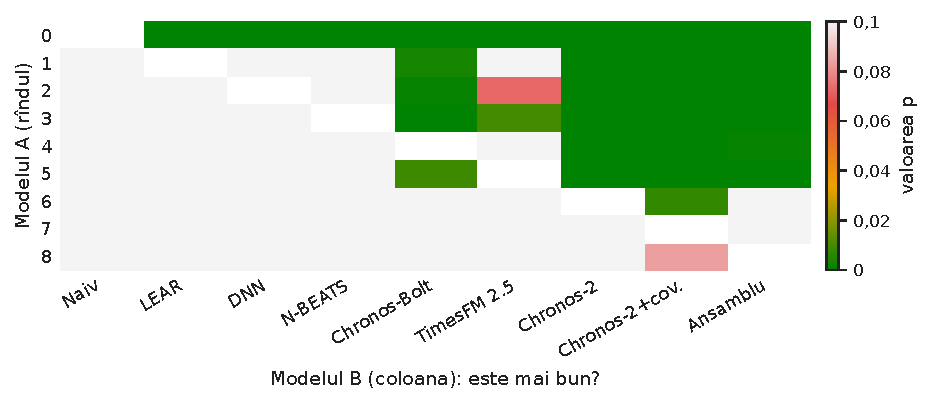
\includegraphics[width=\textwidth,height=0.531\textheight,keepaspectratio]{charts/ro/dm_pvalues.pdf}\end{center}\vspace{-3mm}
\chartsource{Sursa: energy-charts.info (Fraunhofer ISE), din datele burselor și ale ENTSO-E. Date: 1 noiembrie 2025 - 31 octombrie 2026, 360 de zile x 24 de ore, România.}
\vspace{0.5mm}
\begin{itemize}\setlength{\itemsep}{0pt}
  \item Ansamblul față de LEAR: $p$ = $<$0{,}001
    \begin{itemize}\setlength{\itemsep}{0pt}
      \item Ansamblul față de Chronos-2: $p$ = 0{,}565.
    \end{itemize}
\end{itemize}
\par\vfill\noindent{\scriptsize\color{FooterGray}}\hfill\qlink{NN\_L13\_dm\_pvalues}{Quantlets/L13/NN_L13_dm_pvalues}\par\vspace{0.5mm}
\end{frame}


\section{Prognoze probabilistice și calibrare conformală}

\begin{frame}{Prognozele de cuantile se evaluează cu pierderea pinball}
\footnotesize
\intuition{o prognoză de cuantilă este bună cînd sub ea cade proporția corectă de valori, iar banda este îngustă.}
\begin{columns}[T,onlytextwidth]
\begin{column}{0.53\textwidth}
\[ \rho_\tau(u)=u\,\big(\tau-\mathbb 1\{u<0\}\big),\quad u=y-\hat q^{\tau} \]\[ \mathrm{PL}=\frac{1}{9}\sum_{\tau\in\{0.1,\dots,0.9\}}\frac{1}{24|\mathcal T|}\sum_{d,h}\rho_\tau\big(y_{d,h}-\hat q^{\tau}_{d,h}\big) \]{\footnotesize\begin{itemize}\setlength{\itemsep}{0pt}
  \item \textbf{\txtwhere}
    \begin{itemize}\setlength{\itemsep}{0pt}
      \item $\tau$ = nivelul cuantilei
      \item Media pe cele nouă decile aproximează scorul probabilistic continuu (continuous ranked probability score).
    \end{itemize}
\end{itemize}\par}
\end{column}
\begin{column}{0.44\textwidth}
\begin{itemize}\setlength{\itemsep}{2pt}
  \item \textbf{Pierderea pinball medie, anul de test} (EUR/MWh)
    \begin{itemize}\setlength{\itemsep}{0pt}
      \item Chronos-2 8{,}25; cu covariabile 8{,}11
      \item Chronos-Bolt 8{,}62; TimesFM 8{,}97
      \item LEAR + erorile empirice din ultimele 60 de zile 9{,}12
    \end{itemize}
\end{itemize}
\end{column}
\end{columns}
\par\vfill\manager{o baterie sau un departament de risc are nevoie de cuantile
    \begin{itemize}\setlength{\itemsep}{0pt}
      \item Evaluați-le cu pinball, nu cu MAE.
    \end{itemize}}\par\vspace{0.5mm}
\par\vfill\noindent{\scriptsize\color{FooterGray}}\hfill\tryit{notebook \S7}\par\vspace{0.5mm}
\end{frame}

\begin{frame}{O săptămînă de cuantile Chronos-2: banda se lărgește acolo unde prețurile sar}
\small
\intuition{modelul este mai puțin sigur în orele de seară, exact acolo unde erorile sînt cele mai mari.}
\begin{center}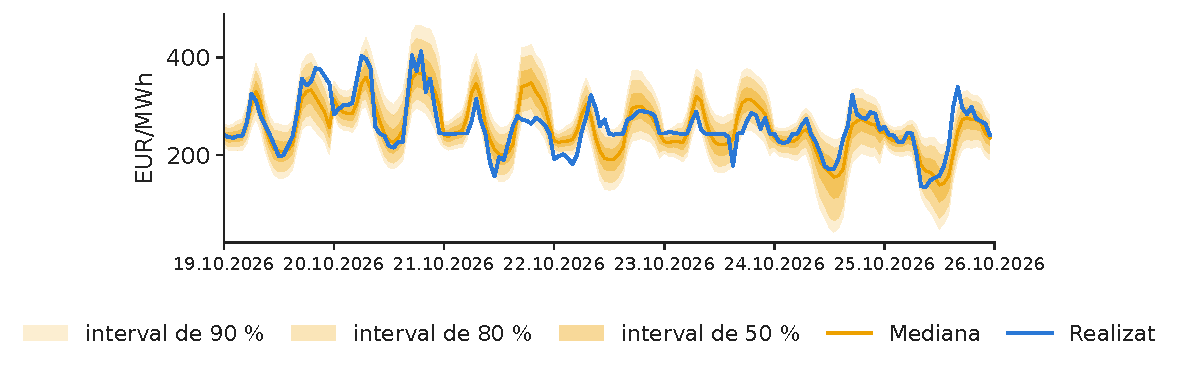
\includegraphics[width=\textwidth,height=0.600\textheight,keepaspectratio]{charts/ro/chronos_fan.pdf}\end{center}\vspace{-3mm}
\chartsource{Sursa: energy-charts.info (Fraunhofer ISE), din datele burselor și ale ENTSO-E. Date: 19 octombrie 2026 - 25 octombrie 2026, orar, România.}
\par\vfill\noindent{\scriptsize\color{FooterGray}}\hfill\qlink{NN\_L13\_chronos\_fan}{Quantlets/L13/NN_L13_chronos_fan}\par\vspace{0.5mm}
\end{frame}

\begin{frame}{Corecția conformală a intervalelor de prognoză}
\footnotesize
\intuition{măsurăm cît de departe de banda brută au căzut valorile în trecutul recent și lărgim (sau îngustăm) banda cu acea valoare.}
\begin{columns}[T,onlytextwidth]
\begin{column}{0.53\textwidth}
\[ s_i=\max\big(\hat q^{\alpha/2}_i-y_i,\ y_i-\hat q^{1-\alpha/2}_i\big),\quad \hat Q=s_{(\lceil (n+1)(1-\alpha)\rceil)} \]\[ \hat C_{d,h}=\big[\hat q^{\alpha/2}_{d,h}-\hat Q,\ \hat q^{1-\alpha/2}_{d,h}+\hat Q\big],\qquad \Pr\big(y\in\hat C\big)\ge 1-\alpha \]{\footnotesize\begin{itemize}\setlength{\itemsep}{0pt}
  \item \textbf{\txtwhere}
    \begin{itemize}\setlength{\itemsep}{0pt}
      \item $s_i$ = scorurile de conformitate pe ultimele 60 de zile ($n$ = 24 $\times$ zile)
      \item $s_{(k)}$ = a $k$-a cea mai mică valoare
      \item Garanția este exactă pentru date interschimbabile și doar aproximativă pentru serii de timp.
    \end{itemize}
\end{itemize}\par}
\end{column}
\begin{column}{0.44\textwidth}
\begin{itemize}\setlength{\itemsep}{2pt}
  \item \textbf{Regresia cuantilă conformală (CQR)} aplicată lui Chronos-2, banda de 80\,\%: acoperire brută 76{,}5\,\%, corectată 79{,}3\,\%.
  \item \textbf{Lățimea}: 60{,}03 $\rightarrow$ 63{,}89 EUR/MWh.
\end{itemize}
\end{column}
\end{columns}
\par\vfill\manager{un model fundație plus calibrarea conformală formează o prognoză probabilistică ieftină și onestă.}\par\vspace{0.5mm}
\par\vfill\noindent{\scriptsize\color{FooterGray}(Romano, Patterson \& Candès, 2019)}\hfill\tryit{notebook \S7}\par\vspace{0.5mm}
\end{frame}

\begin{frame}{Calibrarea conformală aduce acoperirea spre nivelul nominal}
\small
\intuition{liniile negre: nivelul nominal; barele: ponderea orelor de test din interiorul benzii.}
\begin{center}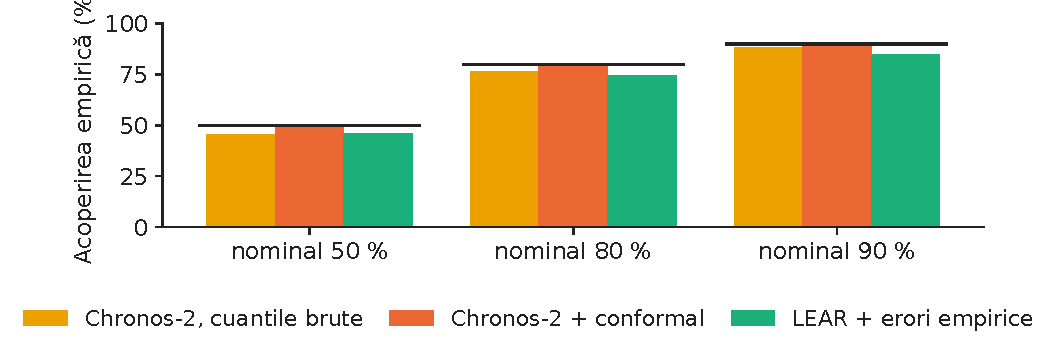
\includegraphics[width=\textwidth,height=0.520\textheight,keepaspectratio]{charts/ro/coverage.pdf}\end{center}\vspace{-3mm}
\chartsource{Sursa: energy-charts.info (Fraunhofer ISE), din datele burselor și ale ENTSO-E. Date: 1 noiembrie 2025 - 31 octombrie 2026, 360 de zile x 24 de ore, România.}
\vspace{0.5mm}
\begin{itemize}\setlength{\itemsep}{0pt}
  \item Banda de 90\,\%: brut 88{,}3\,\%, conformal 89{,}4\,\%, LEAR + erori empirice 85{,}0\,\%
    \begin{itemize}\setlength{\itemsep}{0pt}
      \item TimesFM 80\,\%: brut 79{,}6\,\%, conformal 79{,}7\,\%.
    \end{itemize}
\end{itemize}
\par\vfill\noindent{\scriptsize\color{FooterGray}}\hfill\qlink{NN\_L13\_coverage}{Quantlets/L13/NN_L13_coverage}\par\vspace{0.5mm}
\end{frame}

\begin{frame}{Consumul este mai ușor de prognozat decît prețul: modelele fundație greșesc cu cîteva procente}
\small
\intuition{consumul este neted și sezonier, exact formele pe care un model preantrenat le cunoaște cel mai bine.}
\vspace{-1mm}\[ \mathrm{MAPE}=\frac{100}{24|\mathcal T|}\sum_{d,h}\Big|\frac{\ell_{d,h}-\hat\ell_{d,h}}{\ell_{d,h}}\Big| \]\vspace{-2mm}
\begin{center}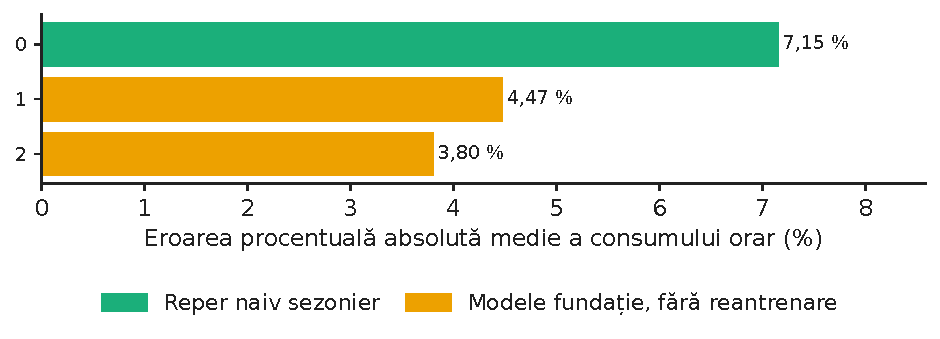
\includegraphics[width=\textwidth,height=0.185\textheight,keepaspectratio]{charts/ro/load_mape.pdf}\end{center}\vspace{-3mm}
\chartsource{Sursa: energy-charts.info (Fraunhofer ISE), din datele burselor și ale ENTSO-E. Date: 1 noiembrie 2025 - 31 octombrie 2026, 360 de zile, consumul României.}
\vspace{0.5mm}
\begin{itemize}\setlength{\itemsep}{0pt}
  \item Eroarea procentuală absolută medie (MAPE): săptămîna trecută 7{,}15\,\%, TimesFM 4{,}47\,\%, Chronos-2 3{,}80\,\% (MAE 214{,}4 MW, consum mediu 5\,932 MW).
\end{itemize}
\par\vfill\manager{erorile procentuale sînt potrivite pentru consum, care nu este niciodată aproape de zero.}\par\vspace{0.5mm}
\par\vfill\noindent{\scriptsize\color{FooterGray}}\hfill\qlink{NN\_L13\_load\_mape}{Quantlets/L13/NN_L13_load_mape}\par\vspace{0.5mm}
\end{frame}


\section{Modele fundație pentru riscul financiar}

\begin{frame}{Valoarea expusă la risc este o cuantilă condiționată, testată prin numărarea depășirilor}
\footnotesize
\intuition{o VaR de 1\,\% trebuie depășită în aproximativ 1\,\% din zile, iar depășirile nu trebuie să vină grupat.}
\begin{columns}[T,onlytextwidth]
\begin{column}{0.53\textwidth}
\[ \Pr\big(r_{t+1}<\mathrm{VaR}^{\alpha}_{t+1}\mid\mathcal F_t\big)=\alpha,\qquad I_{t+1}=\mathbb 1\{r_{t+1}<\mathrm{VaR}^{\alpha}_{t+1}\} \]\[ \mathrm{LR}_{uc}=-2\ln\frac{(1-\alpha)^{n_0}\alpha^{n_1}}{(1-\hat\pi)^{n_0}\hat\pi^{n_1}}\sim\chi^2_1 \]{\footnotesize\begin{itemize}\setlength{\itemsep}{0pt}
  \item \textbf{\txtwhere}
    \begin{itemize}\setlength{\itemsep}{0pt}
      \item $r_t$ = randamentul logaritmic zilnic (\%)
      \item $n_1$ = depășirile, $n_0$ = celelalte zile, $\hat\pi=n_1/(n_0+n_1)$
      \item Testul raportului de verosimilitate (LR) al lui Kupiec
      \item Christoffersen adaugă un test de independență a lui $I_t$.
    \end{itemize}
\end{itemize}\par}
\end{column}
\begin{column}{0.44\textwidth}
\begin{itemize}\setlength{\itemsep}{2pt}
  \item \textbf{Trei metode}
    \begin{itemize}\setlength{\itemsep}{0pt}
      \item Simularea istorică (HS): cuantila empirică a ultimelor 250 de zile
      \item Heteroscedasticitate condiționată autoregresivă generalizată (GARCH): GARCH(1,1) cu erori Student-$t$, reestimat la fiecare 21 de zile
      \item Cuantilele Chronos-2 din ultimele 1.024 de randamente, fără reantrenare
    \end{itemize}
\end{itemize}
\end{column}
\end{columns}
\par\vfill\manager{semaforul Basel depinde de numărul de depășiri ale VaR de 1\,\% în 250 de zile.}\par\vspace{0.5mm}
\par\vfill\noindent{\scriptsize\color{FooterGray}(Kupiec, 1995; Christoffersen, 1998)}\hfill\tryit{notebook \S9}\par\vspace{0.5mm}
\end{frame}

\begin{frame}{O deplasare conformală unilaterală transformă cuantila brută într-o VaR calibrată}
\footnotesize
\intuition{dacă cuantila modelului a fost depășită prea des în ultimul an, o coborîm exact cu valoarea care ar fi corectat-o.}
\begin{columns}[T,onlytextwidth]
\begin{column}{0.53\textwidth}
\[ s_i=\hat q^{\alpha}_i-r_i,\qquad c_t=s_{(\lceil (n+1)(1-\alpha)\rceil)}\ \text{pe ultimele } n=250 \]\[ \widehat{\mathrm{VaR}}^{\alpha}_{t+1}=\hat q^{\alpha}_{t+1}-c_t \]{\footnotesize\begin{itemize}\setlength{\itemsep}{0pt}
  \item \textbf{\txtwhere}
    \begin{itemize}\setlength{\itemsep}{0pt}
      \item $\hat q^{\alpha}$ = cuantila brută Chronos-2
      \item $c_t>0$ mărește VaR, $c_t<0$ o micșorează
      \item Deplasarea folosește doar prognoze și randamente din trecut.
    \end{itemize}
\end{itemize}\par}
\end{column}
\begin{column}{0.44\textwidth}
\begin{itemize}\setlength{\itemsep}{2pt}
  \item \textbf{S\&P 500, nivelul de 1\,\%}: Chronos-2 brut 22 depășiri, conformal 16, așteptate 17{,}2.
  \item \textbf{Aceeași idee} ca la benzile din energie, aplicată unei singure cozi.
\end{itemize}
\end{column}
\end{columns}
\par\vfill\manager{recalibrarea este o schimbare de model: documentați-o și testați-o pe date noi.}\par\vspace{0.5mm}
\par\vfill\noindent{\scriptsize\color{FooterGray}(Romano et al., 2019)}\hfill\tryit{notebook \S9}\par\vspace{0.5mm}
\end{frame}

\begin{frame}{S\&P 500: VaR calibrată a modelului fundație urmărește regimurile de volatilitate}
\small
\intuition{ambele linii se lărgesc în martie 2020 și în aprilie 2025; punctele roșii sînt zilele în care VaR conformală Chronos-2 a fost depășită.}
\begin{center}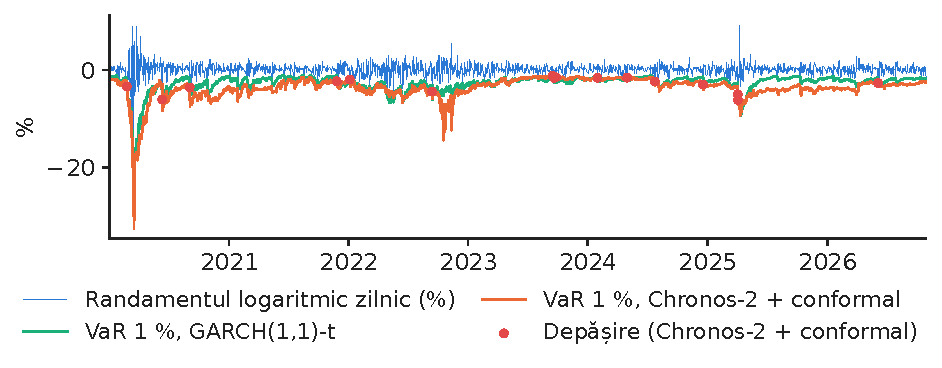
\includegraphics[width=\textwidth,height=0.555\textheight,keepaspectratio]{charts/ro/var_sp500.pdf}\end{center}\vspace{-3mm}
\chartsource{Sursa: Yahoo Finance, cotații zilnice. Date: 2 ianuarie 2020 - 30 octombrie 2026, zile de tranzacționare, S\&P 500.}
\par\vfill\noindent{\scriptsize\color{FooterGray}}\hfill\qlink{NN\_L13\_var\_sp500}{Quantlets/L13/NN_L13_var_sp500}\par\vspace{0.5mm}
\end{frame}

\begin{frame}{Testarea retrospectivă, ianuarie 2020 -- octombrie 2026: S\&P 500 și Bitcoin}
\small
{\scriptsize\renewcommand{\arraystretch}{1.05}\setlength{\tabcolsep}{4pt}
\begin{tabular}{@{}llrrrrrr@{}}\toprule
Activ & Model & Dep.\ 1\,\% & $p_{uc}$ & $p_{ind}$ & Dep.\ 5\,\% & $p_{uc}$ & Pierdere tick 5\,\% \\ \midrule
S\&P 500 & HS (250 de zile) & 31 & \cellcolor{Crimson!52}0{,}003 & 0{,}002 & 89 & \cellcolor{Forest!55}0{,}729 & 0{,}1582 \\
 & GARCH(1,1)-$t$ & 32 & \cellcolor{Crimson!54}0{,}001 & 0{,}607 & 132 & \cellcolor{Crimson!55}0{,}000 & 0{,}1347 \\
 & Chronos-2, brut & 22 & \cellcolor{Forest!55}0{,}262 & 0{,}285 & 122 & \cellcolor{Crimson!55}0{,}000 & 0{,}1368 \\
 & Chronos-2 + conformal & 16 & \cellcolor{Forest!55}0{,}774 & 0{,}138 & 93 & \cellcolor{Forest!55}0{,}434 & 0{,}1383 \\
Bitcoin & HS (250 de zile) & 33 & \cellcolor{Forest!55}0{,}123 & 0{,}458 & 126 & \cellcolor{Forest!55}0{,}912 & 0{,}3633 \\
 & GARCH(1,1)-$t$ & 22 & \cellcolor{Forest!55}0{,}543 & 0{,}189 & 128 & \cellcolor{Forest!55}0{,}770 & 0{,}3587 \\
 & Chronos-2, brut & 31 & \cellcolor{Forest!55}0{,}242 & 0{,}402 & 134 & \cellcolor{Forest!55}0{,}404 & 0{,}3591 \\
 & Chronos-2 + conformal & 21 & \cellcolor{Forest!55}0{,}413 & 0{,}170 & 120 & \cellcolor{Forest!55}0{,}657 & 0{,}3614 \\
\bottomrule\end{tabular}}
\par\vspace{0.5mm}{\scriptsize \begin{itemize}\setlength{\itemsep}{0pt}
  \item Depășiri așteptate: S\&P 500 17{,}2 (1\,\%) și 85{,}9 (5\,\%) în 1\,717 zile; Bitcoin 25{,}0 și 124{,}8 în 2\,496 de zile (tranzacționat zilnic).
  \item Valoare $p$ verde: acoperirea nu este respinsă la 10\,\%; roșie: este respinsă. Pierderea tick = pierderea pinball la $\tau=0{,}05$ (mai mică este mai bine).
\end{itemize}}
\par\vfill\noindent{\scriptsize\color{FooterGray}(calcul propriu; Kupiec, 1995; Christoffersen, 1998)}\hfill\tryit{notebook \S9}\par\vspace{0.5mm}
\end{frame}

\begin{frame}{Prognozele cuantilelor cu modele de limbaj și cu modele de serii de timp}
\small
\begin{itemize}\setlength{\itemsep}{3pt}
  \item \textbf{Calea modelului lingvistic mare (LLM)} (cursul 12)
    \begin{itemize}\setlength{\itemsep}{0pt}
      \item Randamentele sînt scrise ca text într-un prompt; un model general răspunde cu un număr
      \item LLM-VaR și, pentru pierderea așteptată în coada distribuției (ES), LLM-ES, ale grupului nostru: zero-shot, fără ajustare fină (Pele et al., 2026)
    \end{itemize}
  \item \textbf{Calea modelului fundație pentru serii de timp} (acest curs)
    \begin{itemize}\setlength{\itemsep}{0pt}
      \item Numerele intră ca petice scalate; ieșirea este un set de cuantile
      \item Mai ieftin pe prognoză, rulează local, calibrat aici printr-o deplasare conformală
    \end{itemize}
  \item \textbf{Reguli comune}
    \begin{itemize}\setlength{\itemsep}{0pt}
      \item Testați pe date noi, numărați depășirile, testați independența, comparați cu GARCH și HS
    \end{itemize}
\end{itemize}
\end{frame}

\section*{Recapitulare}

\begin{frame}{Test 1: scurgerea de informație}
\small
\begin{itemize}
  \item Un coleg adaugă consumul efectiv al României din ziua $d$ la intrările prognozei de preț pentru ziua $d$, iar MAE scade
    \begin{itemize}\setlength{\itemsep}{0pt}
      \item Puneți modelul în producție?
    \end{itemize}
\end{itemize}
\vspace{2mm}
\begin{exampleblock}{R\u{a}spuns}
\begin{itemize}
  \item Nu: consumul efectiv din ziua $d$ nu se cunoaște la ora 12:00 din ziua $d-1$
    \begin{itemize}\setlength{\itemsep}{0pt}
      \item Folosiți prognoza operatorului sau decalaje disponibile la închiderea licitației.
    \end{itemize}
\end{itemize}
\end{exampleblock}
\end{frame}

\begin{frame}{Test 2: lățimea conformală}
\small
\begin{itemize}
  \item Banda brută de 80\,\% a lui Chronos-2 a acoperit 76{,}5\,\% din orele de test
    \begin{itemize}\setlength{\itemsep}{0pt}
      \item Ce face pasul conformal cu lățimea ei și de ce?
    \end{itemize}
\end{itemize}
\vspace{2mm}
\begin{exampleblock}{R\u{a}spuns}
\begin{itemize}
  \item O modifică cu $\hat Q$, cuantila de nivel $(1-\alpha)$ a distanțelor recente în afara benzii: o lărgește dacă banda era prea îngustă și o îngustează dacă era prea largă (aici 60{,}03 $\rightarrow$ 63{,}89 EUR/MWh).
\end{itemize}
\end{exampleblock}
\end{frame}

\begin{frame}{Test 3: testul Kupiec}
\small
\begin{itemize}
  \item În 1\,717 zile, o VaR de 1\,\% a avut de 3 ori numărul așteptat de depășiri
    \begin{itemize}\setlength{\itemsep}{0pt}
      \item Valoarea $p$ a testului Kupiec este mare sau mică?
    \end{itemize}
\end{itemize}
\vspace{2mm}
\begin{exampleblock}{R\u{a}spuns}
\begin{itemize}
  \item Mică: $\hat\pi$ este departe de $\alpha$, deci $\mathrm{LR}_{uc}$ este mare și acoperirea se respinge
    \begin{itemize}\setlength{\itemsep}{0pt}
      \item Modelul subestimează riscul.
    \end{itemize}
\end{itemize}
\end{exampleblock}
\end{frame}

\begin{frame}{Recapitulare}
\small
\begin{itemize}\setlength{\itemsep}{4pt}
  \item Mai întîi reperele: naiv 27{,}74, LEAR 22{,}79 EUR/MWh
    \begin{itemize}\setlength{\itemsep}{0pt}
      \item Cea mai mică MAE: Chronos-2 cu covariabile (20{,}41).
    \end{itemize}
  \item Modelele fundație prognozează prețul și consumul fără reantrenare
    \begin{itemize}\setlength{\itemsep}{0pt}
      \item Lungimea contextului și covariabilele sînt parametrii lor de ajustare.
    \end{itemize}
  \item Semnificația, prin testul Diebold--Mariano pe pierderile zilnice
    \begin{itemize}\setlength{\itemsep}{0pt}
      \item Mai multe rulări pentru fiecare rețea.
    \end{itemize}
  \item Calibrarea conformală transformă cuantilele brute în benzi și VaR oneste
    \begin{itemize}\setlength{\itemsep}{0pt}
      \item Testați retrospectiv cu Kupiec și Christoffersen.
    \end{itemize}
  \item Urmează: modelele multimodale și sinteza cursului (cursul 14).
\end{itemize}
\end{frame}

\begin{frame}{Cercetările grupului nostru}
\footnotesize
\begin{itemize}\setlength{\itemsep}{3pt}
  \item \textbf{Patru generații de metode de prognoză a prețurilor energiei}: modele econometrice, învățare automată, LSTM și arhitecturi transformer, comparate pe piețele europene de energie, inclusiv preantrenarea și transferul învățării (Andrei, Velev, Toma, Pele \& Lessmann, 2024, arXiv 2411.03372).
  \item \textbf{Avertizarea timpurie a vîrfurilor de preț}: modele explicabile de tip gradient boosting pe date orare din România
    \begin{itemize}\setlength{\itemsep}{0pt}
      \item Prognoza sarcinii reziduale este principalul declanșator al avertizărilor (Andrei, Pele, Cramer, Amza \& Diaconu, 2026, PICBE).
    \end{itemize}
  \item \textbf{Explicabilitate pe mai multe orizonturi}: ce factori contează de la 0--6 ore pînă la două săptămîni și în ce regim de preț, România 2018--2024 (Andrei, Pele \& Cramer, 2026, PICBE).
  \item \textbf{LLM-VaR și LLM-ES}: modele de limbaj generale produc, fără reantrenare, prognoze ale valorii expuse la risc și ale pierderii așteptate în coada distribuției (ES) pe baza unui prompt cu randamentele trecute (Pele et al., 2026, Expert Systems with Applications).
  \item \textbf{Avertizare timpurie pentru criptoactivele „zombie”}: învățarea automată prezice care criptoactive vor deveni inactive (Będowska-Sójka, Wójcik \& Pele, 2026, North American Journal of Economics and Finance).
\end{itemize}
\par\vspace{0.5mm}{\scriptsize \begin{itemize}\setlength{\itemsep}{0pt}
  \item Rezultatele sînt preluate din rezumatele lucrărilor; cifrele de pe celelalte slide-uri provin din datele noastre.
\end{itemize}}
\par\vfill\noindent{\scriptsize\color{FooterGray}(Academia de Studii Economice din București, ASE; Academia Română, Institutul de Prognoză Economică, IPE)}\par\vspace{0.5mm}
\end{frame}

\begin{frame}{Lecturi și resurse suplimentare}
\small
\begin{columns}[T,onlytextwidth]
\begin{column}{0.5\textwidth}
\begin{itemize}\setlength{\itemsep}{4pt}
  \item \textbf{Chronos}, cod și modele: \href{https://github.com/amazon-science/chronos-forecasting}{github.com/amazon-science/chronos-forecasting}.
  \item \textbf{TimesFM}: \href{https://github.com/google-research/timesfm}{github.com/google-research/timesfm}.
  \item \textbf{epftoolbox}, reperul deschis al lui Lago et al.\ (2021): \href{https://github.com/jeslago/epftoolbox}{github.com/jeslago/epftoolbox}.
\end{itemize}
\end{column}
\begin{column}{0.47\textwidth}
\begin{itemize}\setlength{\itemsep}{4pt}
  \item \textbf{Predicția conformală}, o introducere accesibilă: \href{https://arxiv.org/abs/2107.07511}{arXiv:2107.07511}.
  \item \textbf{Forecasting: Principles and Practice}, ed.\ a 3-a: \href{https://otexts.com/fpp3/}{otexts.com/fpp3}.
  \item \textbf{Acest curs}: notebook, seminar și Quantlets --- \href{https://github.com/danpele/NEURAL_BIZ}{github.com/danpele/NEURAL\_BIZ}.
\end{itemize}
\end{column}
\end{columns}
\end{frame}

\begin{frame}{Bibliografie (1/2)}
\scriptsize
\begin{itemize}\setlength{\itemsep}{0pt}\scriptsize
\item Andrei, A.-V., Pele, D.-T., Cramer, A.-A., Amza, A.\ \& Diaconu, D.\ (2026). Explainable AI-based early warning system for electricity price spikes: Evidence from the Romanian market. \textit{Proceedings of the International Conference on Business Excellence}, 20(1), 4820--4836. \href{https://doi.org/10.2478/picbe-2026-0352}{doi:10.2478/picbe-2026-0352}
\item Andrei, A.-V., Pele, D.-T.\ \& Cramer, A.-A.\ (2026). Multi-horizon explainability in energy price forecasting: Disentangling market dynamics and renewable intermittency in Romania's liberalized electricity market. \textit{Proceedings of the International Conference on Business Excellence}, 20(1), 104--117. \href{https://doi.org/10.2478/picbe-2026-0014}{doi:10.2478/picbe-2026-0014}
\item Andrei, A.-V., Velev, G., Toma, F.-M., Pele, D.\,T.\ \& Lessmann, S.\ (2024). Energy price modelling: A comparative evaluation of four generations of forecasting methods. \href{https://arxiv.org/abs/2411.03372}{arXiv:2411.03372}
\item Ansari, A.\,F.\ et al.\ (2024). Chronos: Learning the language of time series. \textit{Transactions on Machine Learning Research}. \href{https://arxiv.org/abs/2403.07815}{arXiv:2403.07815}
\item Ansari, A.\,F.\ et al.\ (2025). Chronos-2: From univariate to universal forecasting. \href{https://arxiv.org/abs/2510.15821}{arXiv:2510.15821}
\item Będowska-Sójka, B., Wójcik, P.\ \& Pele, D.\,T.\ (2026). Early warning systems for cryptocurrency markets: Predicting `zombie' assets using machine learning. \textit{The North American Journal of Economics and Finance}, 81, 102543. \href{https://doi.org/10.1016/j.najef.2025.102543}{doi:10.1016/j.najef.2025.102543}
\item Christoffersen, P.\,F.\ (1998). Evaluating interval forecasts. \textit{International Economic Review}, 39(4), 841--862. \href{https://doi.org/10.2307/2527341}{doi:10.2307/2527341}
\item Das, A., Kong, W., Sen, R.\ \& Zhou, Y.\ (2024). A decoder-only foundation model for time-series forecasting. \textit{Proceedings of the 41st International Conference on Machine Learning}. \href{https://arxiv.org/abs/2310.10688}{arXiv:2310.10688}
\item Diebold, F.\,X.\ \& Mariano, R.\,S.\ (1995). Comparing predictive accuracy. \textit{Journal of Business \& Economic Statistics}, 13(3), 253--263. \href{https://doi.org/10.1080/07350015.1995.10524599}{doi:10.1080/07350015.1995.10524599}
\item Kupiec, P.\,H.\ (1995). Techniques for verifying the accuracy of risk measurement models. \textit{The Journal of Derivatives}, 3(2), 73--84. \href{https://doi.org/10.3905/jod.1995.407942}{doi:10.3905/jod.1995.407942}
\end{itemize}
\end{frame}

\begin{frame}{Bibliografie (2/2)}
\scriptsize
\begin{itemize}\setlength{\itemsep}{0pt}\scriptsize
\item Lago, J., Marcjasz, G., De Schutter, B.\ \& Weron, R.\ (2021). Forecasting day-ahead electricity prices: A review of state-of-the-art algorithms, best practices and an open-access benchmark. \textit{Applied Energy}, 293, 116983. \href{https://doi.org/10.1016/j.apenergy.2021.116983}{doi:10.1016/j.apenergy.2021.116983}
\item Nie, Y., Nguyen, N.\,H., Sinthong, P.\ \& Kalagnanam, J.\ (2023). A time series is worth 64 words: Long-term forecasting with transformers. \textit{International Conference on Learning Representations}. \href{https://arxiv.org/abs/2211.14730}{arXiv:2211.14730}
\item Oreshkin, B.\,N., Carpov, D., Chapados, N.\ \& Bengio, Y.\ (2020). N-BEATS: Neural basis expansion analysis for interpretable time series forecasting. \textit{International Conference on Learning Representations}. \href{https://arxiv.org/abs/1905.10437}{arXiv:1905.10437}
\item Pele, D.\,T., Bolovăneanu, V., Lin, M.-B., Ren, R., Ginavar, A.\,T., Spilak, B., Andrei, A.-V., Toma, F.-M., Lessmann, S.\ \& Härdle, W.\,K.\ (2026). In the beginning was the Word: LLM-VaR and LLM-ES. \textit{Expert Systems with Applications}, 295, 128676. \href{https://doi.org/10.1016/j.eswa.2025.128676}{doi:10.1016/j.eswa.2025.128676}
\item Romano, Y., Patterson, E.\ \& Candès, E.\ (2019). Conformalized quantile regression. \textit{Advances in Neural Information Processing Systems}, 32. \href{https://arxiv.org/abs/1905.03222}{arXiv:1905.03222}
\item Salinas, D., Flunkert, V., Gasthaus, J.\ \& Januschowski, T.\ (2020). DeepAR: Probabilistic forecasting with autoregressive recurrent networks. \textit{International Journal of Forecasting}, 36(3), 1181--1191. \href{https://doi.org/10.1016/j.ijforecast.2019.07.001}{doi:10.1016/j.ijforecast.2019.07.001}
\item Uniejewski, B., Weron, R.\ \& Ziel, F.\ (2018). Variance stabilizing transformations for electricity spot price forecasting. \textit{IEEE Transactions on Power Systems}, 33(2), 2219--2229. \href{https://doi.org/10.1109/TPWRS.2017.2734563}{doi:10.1109/TPWRS.2017.2734563}
\item Weron, R.\ (2014). Electricity price forecasting: A review of the state-of-the-art with a look into the future. \textit{International Journal of Forecasting}, 30(4), 1030--1081. \href{https://doi.org/10.1016/j.ijforecast.2014.08.008}{doi:10.1016/j.ijforecast.2014.08.008}
\item Ziel, F.\ \& Weron, R.\ (2018). Day-ahead electricity price forecasting with high-dimensional structures: Univariate vs.\ multivariate modeling frameworks. \textit{Energy Economics}, 70, 396--420. \href{https://doi.org/10.1016/j.eneco.2017.12.016}{doi:10.1016/j.eneco.2017.12.016}
\end{itemize}
\end{frame}

\appendix

\section*{Anexă}

\begin{frame}{Anexa A: de ce acoperă banda conformală}
\small
\begin{itemize}\setlength{\itemsep}{4pt}
  \item Fie $s_1,\dots,s_n,s_{n+1}$ scoruri de conformitate interschimbabile
    \begin{itemize}\setlength{\itemsep}{0pt}
      \item Rangul lui $s_{n+1}$ printre ele este uniform pe $\{1,\dots,n+1\}$.
    \end{itemize}
  \item De aici $\Pr(s_{n+1}\le s_{(k)})\ge k/(n+1)$
    \begin{itemize}\setlength{\itemsep}{0pt}
      \item Alegînd $k=\lceil (n+1)(1-\alpha)\rceil$ obținem $\Pr(s_{n+1}\le\hat Q)\ge 1-\alpha$.
    \end{itemize}
  \item $s_{n+1}\le\hat Q$ este echivalent cu $y_{n+1}\in[\hat q^{\alpha/2}-\hat Q,\hat q^{1-\alpha/2}+\hat Q]$, adică banda.
  \item Orele unei serii de prețuri sînt dependente și au derivă
    \begin{itemize}\setlength{\itemsep}{0pt}
      \item Fereastra glisantă de 60 de zile renunță la exactitate în favoarea adaptării.
    \end{itemize}
\end{itemize}
\par\vfill\noindent{\scriptsize\color{FooterGray}(Romano, Patterson \& Candès, 2019)}\par\vspace{0.5mm}
\end{frame}

\begin{frame}{Anexa B: testul de independență al lui Christoffersen}
\small
\begin{itemize}\setlength{\itemsep}{4pt}
  \item Numărăm tranzițiile șirului de depășiri: $n_{ij}$ = numărul de zile cu $I_{t-1}=i$ și $I_t=j$
    \begin{itemize}\setlength{\itemsep}{0pt}
      \item $\hat\pi_{01}=n_{01}/(n_{00}+n_{01})$, $\hat\pi_{11}=n_{11}/(n_{10}+n_{11})$.
    \end{itemize}
  \item $\mathrm{LR}_{ind}=-2\ln\frac{(1-\hat\pi)^{n_{00}+n_{10}}\hat\pi^{n_{01}+n_{11}}}{(1-\hat\pi_{01})^{n_{00}}\hat\pi_{01}^{n_{01}}(1-\hat\pi_{11})^{n_{10}}\hat\pi_{11}^{n_{11}}}\sim\chi^2_1$.
  \item O valoare $p$ mică înseamnă că depășirile vin grupat: modelul reacționează prea încet la un șoc de volatilitate.
\end{itemize}
\par\vfill\noindent{\scriptsize\color{FooterGray}(Christoffersen, 1998)}\par\vspace{0.5mm}
\end{frame}

\begin{frame}{Anexa C: detalii de implementare}
\small
\begin{itemize}\setlength{\itemsep}{4pt}
  \item LEAR: LassoLarsIC din scikit-learn (criteriul AIC), intrări standardizate, reestimare zilnică pe 1\,092 de zile.
  \item DNN și N-BEATS: PyTorch, pierdere L1, Adam, oprire timpurie
    \begin{itemize}\setlength{\itemsep}{0pt}
      \item Valorile generatorului aleator: 20261108 și următoarele.
    \end{itemize}
  \item Modelele fundație: amazon/chronos-2, amazon/chronos-bolt-base, google/timesfm-2.5-200m-pytorch de pe Hugging Face, doar inferență
    \begin{itemize}\setlength{\itemsep}{0pt}
      \item Rularea completă a durat 2{,}7 minute pe un laptop.
    \end{itemize}
  \item Orele urmează calendarul CET
    \begin{itemize}\setlength{\itemsep}{0pt}
      \item Ora dublă din toamnă este mediată
      \item Zilele cu o oră lipsă sînt excluse din țintele de antrenare și din test.
    \end{itemize}
\end{itemize}
\end{frame}

\end{document}
